
\chapter{Function Merging for Free} \label{chp:lctes21}


\renewcommand{\ProjName}{{HyFM}\xspace}
\newcommand{\SOAName}{{SalSSA}\xspace}
\newcommand{\NW}{{Needleman-Wunsch}\xspace}


%The current state-of-the-art, {\SOAName}~\cite{rocha19,rocha20}, 
%The technique proposed in Chapter~\ref{chp:pldi20}, {\SOAName}, achieves on average a 10\% code size reduction but at the cost of crippling compile-time inefficiencies for large programs.
The technique proposed in Chapter~\ref{chp:pldi20}, {\SOAName}, can lead to 40\% slower compilation, taking up to 32~GB of memory for temporary data when compiling a modestly-sized program.
Such a resource requirement is beyond what is typically available to a developer and thus unsuitable for optimizing real-life programs.
%assuming the development system has that much available memory to begin with.

These inefficiencies stem directly from {\SOAName}'s core innovation, i.e., the sequence alignment algorithm used to identify mergeable instructions in a pair of input functions.
The alignment algorithm has quadratic time and space complexity, so applying it on whole functions with thousands of instructions results in unacceptable overheads.
This severely limits the applicability of function merging on relatively large programs.
%A different function merging approach that delivers similarly high code size reduction without the overheads is necessary.
To make function merging scalable and practical, we need to find ways to significantly reduce the memory and compilation overhead. Our work is designed to offer such capabilities.   

%However, given its powerful capability for code size reduction, we need function merging techniques with acceptable compilation overheads.
%and it might even make it a bad idea for use on smaller programs.
%In either case, making it part of a standard compiler optimization sequence is inadvisable.
%\fixme{MC: you could be stronger here, it's not like the SalSSA people are going to review it}

In this chapter, we present \ProjName, a novel function merging technique that addresses the performance inefficiencies of \SOAName.
Our main insight is that most of the code reduction of {\SOAName} comes from matching highly similar basic blocks.
Even though it is able to align arbitrary subsequences spanning basic block boundaries, profitable alignments usually contain instructions from one block matched to instructions from a single other block.
%The quadratic alignment algorithm, while in principle able to align subsequences spanning basic block boundaries, usually ends up aligning instructions from one block to instructions from a single other block.
We show that an approach which quickly identifies similar basic blocks and then aligns their short instruction sequences achieves a similar code reduction for a much lower overhead.

More specifically, our solution is three fold:
\begin{itemize} %[noitemsep,topsep=3pt]
   \item We align the input functions on a per basic block manner.
   % PP: The fingerprint bit is a detail that we have not discussed and the reviewer might not understand its meaning. Also are contribution regarding fingerprints is minimal.
   First, we pair similar basic blocks by minimizing the distance between their fingerprints.
   Then, we only align the instructions within each pair of basic block.  
   Even with a quadratic alignment algorithm, basic blocks are usually much shorter than functions, translating into a much faster alignment.
   \item We propose a linear pairwise alignment as an alternative to the quadratic one. For highly similar basic blocks, it achieves similar results but has negligible time and space overheads.
   \item We estimate the profitability of the aligned basic blocks before actually generating their merged code.
   If unprofitable, we ignore them, improving the overall profitability of the whole merged function and simplifying code generation.
   If all paired blocks in a pair of functions are unprofitable, we skip merging the function pair altogether, speeding up the optimization process compared to {\SOAName}. 
\end{itemize}

Experimental results on SPEC CPU 2006 and 2017 show that {\ProjName} runs over 4.5$\times$ faster than {\SOAName}.
%reducing end-to-end compilation time by up to \fixme{18}\%.
%Such a fast function merging technique translates to a 
Compared to a baseline without function merging, {\ProjName} reduces end-to-end compilation time by up to 18\% and 2.1\% on average.
%This reduction on end-to-end compilation time is possible due to 
%In most cases the time overhead of our approach is comparable to the speedup experienced by later compilation stages due to the reduced amount of code, making applying {\ProjName} time-neutral.
{\ProjName} also has orders of magnitude lower peak memory usage, using up to 48~MB or 5.6~MB, depending on the variant used, while {\SOAName} requires 32~GB in the worst case.
We achieve all these compilation-time benefits without degrading its ability to reduce code size.


\section{Background and Motivation} \label{sec:motivation}

%In this section, we discuss the key weaknesses of the state-of-the-art function merging, called {\SOAName}~\cite{rocha20}, addressed in this paper.
%First, we show how different stages in {\SOAName} impact its running time.
%\textbf{TODO: Memory usage.}

%In this section, we will discuss how different stages of the state-of-the-art function merging impact during compilation time.
%present how different stages of the state-of-the-art function merging impact its running time.
%In this section, we will present how sequence alignment can be an important source of compilation time overhead.
%Then we discuss how we can address this issue by doing less work, while still keeping most of the code size reduction from the state-of-the-art technique.

In this section, we first provide an overview of the working mechanism of \SOAName, described in Chapter~\ref{chp:pldi20}. We highlight the main drawbacks of \SOAName in terms of compile time and memory footprint. We then outline how we can address these drawbacks without compromising on code size reduction. 

\subsection{Function Merging via Sequence Alignment}
Existing function merging techniques consist of three major stages: choosing which functions to merge, producing the merged function, and estimating the merging profitability.
%\fixme{PP: Is it accurate to talk about two major stages in SalSSA and also this being the case for most optimizations?}

In order to pair similar functions for merging, \SOAName employs a ranking strategy based on the similarity of the \textit{fingerprints} of the functions.
A fingerprint summarizes the content of a function as a fixed-size vector of the frequency of each LLVM-IR opcode. The representation allows the compiler to compare functions using a simple distance metric, such as the Manhattan distance. For a given reference function, all other functions are ranked based on their distance and the closest function is chosen for merging.

Merging two functions requires identifying similar code segments in the two functions that can be profitably merged.
The main innovation of \SOAName~\cite{rocha20} and its predecessor~\cite{rocha19} is the use of a sequence alignment algorithm, called the \NW algorithm, for identifying similar code segments.
This allows them to merge arbitrary pairs of functions.
First, they transform each function into a linear sequence of labels and instructions.
Then, the alignment algorithm is applied on the sequences of the whole input functions.
The resulting alignment is used to generate the merged function.
Once the merged function has been generated, they apply an SSA reconstruction algorithm.
For a final clean up, they simplify the merged function by removing redundant instructions introduced by function merging.
% PP: still not sure that this information is useful for understanding our contribution

Finally, a profitability analysis estimates the benefit of replacing the original pair of functions with the simplified merged function. If unprofitable, the merged function is simply thrown away. Otherwise, they delete the original functions, redirecting the calls to the merged function.
%If the original functions cannot be deleted, e.g., because they might be called externally, their body is replaced by a call to the merged function.
% PP: Similarly not really important for understanding our contribution

\subsection{Limitations of The State of The Art}
%PP: I think we should reorganise this a bit. After refocusing the discussion here on memory, jumping to a subsection called "Compilation Overhead Breakdown" that mainly talks about compilation time seems disconnected. Instead, we should merge the two subsection making the first half about the limitations in terms of memory and the second about the limitations in terms of runtime.

When reproducing the {\SOAName} experiments using the available artifact~\cite{rocha20} on our machine, we were unable to build \texttt{602.gcc\_s}, from SPEC 2017, due to an out of memory crash. 16~GB of memory were not enough for {\SOAName}. 
We succeeded only after migrating to a 64~GB machine which could fit the 32~GB of temporary data produced by function merging.
After investigating further, we realized that this is due to the quadratic algorithm used for aligning the two functions selected for merging.
Because this algorithm is applied on the linearized sequences of the whole input functions, \SOAName incurs a high memory footprint when merging even medium sized functions.
For larger ones, it is impossible to apply it on most workstations or even many servers, making {\SOAName} impractical for use in production.
%For the same reason, alignment brings the compilation process to a crawl for large functions.


%\subsection{Compilation Overhead Breakdown}
\label{sec:motivation:breakdown}

%When merging two functions, the goal is to identify which segments of the code are different and which ones are equivalent, and therefore mergeable.
%To this end, SalSSA uses an optimal sequence alignment algorithm, called the Needleman-Wunsch algorithm, which is quadratic on the size of the input sequences.
%Since SalSSA applies it on the linearised sequences of the whole input functions, the time spend aligning sequences can be significant for programs with very large functions.

For the same reason, alignment brings the compilation process to a crawl for large functions.
Figure~\ref{fig:compilation-breakdown-motivation-alignment} shows the running time breakdown for the different stages of the function merging pass in the LLVM-based \SOAName  implementation for two SPEC CPU2017 benchmarks. 
Sequence alignment dominates the running time of function merging, representing up to 83\% of its overall running time. 
Sequence alignment alone takes 25 seconds and 4.2 minutes on \texttt{638.imagick\_s} and \texttt{602.gcc\_s}, respectively.
%PP: Remove the next sentence?
The alignment stage also causes the peak in memory usage for these two programs, 4.5~GB for \texttt{638.imagick\_s} and 32~GB for \texttt{602.gcc\_s}.
This is not surprising, as the Needleman-Wunsch algorithm has a quadratic complexity in both time and memory usage.
Because this algorithm is applied on linearized sequences of the whole input functions, programs containing large functions, such as the ones in our example, are heavily affected.
%For example, \texttt{638.imagick\_s} has a total of 15,454 functions with the largest one having 73,127 instructions.
%Meanwhile, even though \texttt{602.gcc\_s} has only 2,457 functions, its largest function has 28,974 instructions; hence \SOAName also incurs significant peak memory usage when processing this program. 

\begin{figure}[h]
  \centering
  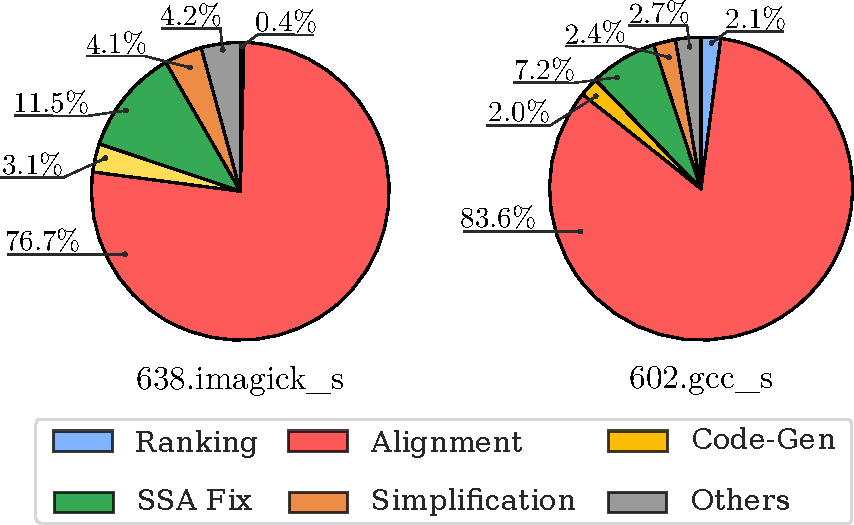
\includegraphics[width=0.7\linewidth]{src/lctes21/figs/compilation-breakdown-motivation-alignment.pdf}
  \caption{Breakdown of the relative runtime for the different stages from {\SOAName}. Alignment takes 25 seconds and 4.2 minutes on \texttt{638.imagick\_s} and \texttt{602.gcc\_s}, respectively.}
  \label{fig:compilation-breakdown-motivation-alignment}
\end{figure}

Most of the rest of the running time of function merging is associated with producing merged functions from the aligned sequences.
%\fixme{PP: Same suggestion as earlier about CodeGen.}
This includes the time spent on the code generation stage (Code-Gen), SSA reconstruction (SSA Fix), and code simplification (Simplification). These stages account for 18.7\% of the {\SOAName}’s running time on \texttt{638.imagick\_s} and 11.6\% on \texttt{602.gcc\_s}.
However, for other programs, these stages may represent the vast majority of {\SOAName}’s running time (see Section~\ref{sec:eval:pass-speedup}).

This breakdown includes the cost for producing both \emph{profitable} and \emph{unprofitable} merged functions.
In fact, most of it is wasted on merged functions that will be rejected by the profitability analysis.
These costs are pronounced because unprofitably merged functions have no limit on their size or complexity, often adding a significant pressure on the SSA reconstruction and simplification stages.
This effect is tied to the alignment strategy, since a good alignment is needed for producing profitably merged functions.
As we discuss in Section~\ref{sec:motivation:less-more}, a better approach would include a finer grain profitability analysis that would allows us to bail out from merging complex and unprofitable code as early as possible.

\subsection{When Less is More} \label{sec:motivation:less-more}

We observe that most of the benefit of function merging often comes from merging highly similar, but not necessarily identical, basic blocks. Figure~\ref{fig:xalan-example} shows one such example extracted from the \texttt{483.xalancbmk} benchmark found in SPEC CPU2006.
This example shows the two input functions annotated with the alignment produced by \SOAName. Merging these two functions contributes to a reduction of 33 bytes in the final object file.

\begin{figure}[h]
  \centering
  \includegraphics[width=\linewidth]{src/lctes21/figs/xalan-example.pdf}
  \caption{Example extracted from \texttt{483.xalancbmk} in SPEC CPU2006. Instructions marked green have been aligned through sequence alignment with an instruction from the other function. {\SOAName} would attempt merging all matched instructions but only the ones in fully aligned basic blocks would be profitable.}
  \label{fig:xalan-example}
\end{figure}

% \begin{figure*}[h]
%   \centering
%   \includegraphics[width=0.6\textwidth]{figs/xalan-example.pdf}
%   \caption{Example extracted from \texttt{483.xalancbmk} found in SPEC CPU2006.}
%   \label{fig:xalan-example}
% \end{figure*}

%This example also suggests that 
While this approach is flexible enough to identify very complex alignments, what it actually produces is three aligned pairs of basic blocks and a few aligned instructions in the entry blocks. More importantly, these entry block instructions offer nothing in terms of code size reduction. The gains of merging them are negated by the extra branches and operand selections needed to preserve the program's semantics. Since {\SOAName} analyzes the profitability of the final merged function as a whole, this unprofitable sequence of instructions will be merged because of the three highly profitable basic blocks. For the same reason, we may have profitable areas of code rejected because the rest of the merged function is unprofitable.


%Since {\SOAName} analyzes the profitability of the final merged function as a whole, we may have segments of unprofitably merged code inside an otherwise profitably merged function.
%Similarly, we may also have segments of profitably merged code inside merged functions that are thrown away by the profitability analysis. 
%However, we can achieve the same code size reduction of 33 bytes by merging only the subset of nearly identical basic blocks (highlighted in Figure~\ref{fig:xalan-example}).
%The gains of merging the entry blocks are negated by the extra branches and operand selections needed to preserve the program's semantics.

This example shows us that we could achieve similar code size reduction by breaking the problem of aligning functions into two simpler processes: first identifying highly similar basic blocks and then aligning the instructions in each pair of similar blocks. 
%merging functions on the basic block rather than on the instruction level adopted by \SOAName.
By operating on basic blocks, we could greatly reduce the length of the sequences to be aligned and the associated compilation and memory overhead. Furthermore, by making profitability decisions for each pair of basic blocks separately, we could avoid merging unprofitable pairs. The rest of this chapter shows how we use such an approach to overcome the weaknesses of \SOAName and make function merging practical for optimizing large programs. 

%Therefore, the main takeaways are:
%1) It often suffices to merge functions on a per basic block manner. %, since crossing the basic block boundary is rarely necessary.
%2) A fine-grain profitability analysis is needed to avoid  merging unprofitable pairs of basic blocks.



%This happens because the optimal sequence alignment algorithm used by SalSSA is trying to maximize the number of matching entries, which does not necessarily translate to the optimal merged function.
%Moreover, SalSSA is also limited by the fixed linearization strategy.
%For example, the two \textit{return} instructions are not aligned due to the ordering of the basic blocks chosen by the linearization strategy.

%We can take advantage of this insight in order to design a faster function merging technique.
%Ultimately, our goal is to be able to avoid the quadratic algorithm while still producing significant reductions to the program's size.

%In this paper, we take advantage of these key insights to propose a novel function merging technique that addresses the major overheads discussed in Section~\ref{sec:motivation:breakdown}.
%We can take advantage of this insight in order to design a better and faster function merging technique.
%To this end, we propose a novel function merging technique that work on the level of basic blocks and includes a fine-grain profitability analysis.



%bail out early from   of a fine-grain and a coarse-grain analysis.

%TODO: [Relatedwork] Note that this is different from the work done by von Koch~et~al.~\cite{edler14}, as these two functions are not \textit{structurally similar} as expected by their function merging technique and therefore could not be merged.


\section{Hybrid Function Merging} \label{sec:contribution}

In this section, we propose {\ProjName} (Hybrid Function Merging), a novel function merging technique that can operate on all functions regardless of their size with little to no compilation overheads.
%and introduces little to no end-to-end overhead, while still delivering similar or better code size reduction as the state-of-the-art.
To achieve this goal, we rely on the insights discussed in Section~\ref{sec:motivation}.
Our solution is three-fold:
1) We introduce an alignment strategy that works on the level of basic blocks, without crossing their boundaries, leading to faster and less memory demanding alignment;
2) We incorporate a multi-tier profitability analysis that allows us to bail out from unprofitable merging attempts even before code generation;
3) We introduce a linear pairwise alignment for basic blocks of the same size that produces good results on highly similar blocks.
This technique can be enabled as an alternative to the quadratic sequence alignment algorithm.
Both techniques have their place, offering different trade-offs.
%\fixme{MC: Saying "propose" here sounds a bit passive compared to the previous two points. Better to say "introduce" then make it clear that it is a complementary technique to NM, and both may have their place}

\subsection{Overview}

For all candidate functions and basic blocks, we generate a fixed-vector representation, namely, their fingerprint~\cite{rocha19,rocha20}.
We match each function with its most similar available function, the one with the shortest fingerprint distance.
Instead of aligning their linearized representations directly, we work at the basic block level.
We pair similar basic blocks of the two functions based on their fingerprint distances.
%Unlike prior work, we require no linearization of the input functions.
We align the instructions in these paired basic blocks using either the {\NW} alignment~\cite{needleman70} or our linear pairwise alignment strategy.
We employ the first-tier profitability analysis on each alignment. If the cost model deems it unprofitable, we skip the pair.
The pairing of basic blocks, the alignment, and the first-tier profitability analysis are executed in rounds, in a greedy manner.
That is, the first profitable pairing is taken, however, unprofitable paired blocks are freed for another pairing, if necessary.
%\fixme{PP: We should mention this in 3.2, 3.3, or 3.4 too. Also how does that work when we have no first-tier profitability analysis? Do we always keep the first pair or do we keep merging the functions and doing the second tier analysis for every single basic block pair we try?}

Once all basic blocks have been processed, we combine the block alignments into a function-wide one and we produce the merged function using the same code generation proposed for {\SOAName}~\cite{rocha20}.
If no profitable pair of basic blocks was found, we bail out before code generation.
Finally, we perform the second-tier profitability analysis, which is the same used by {\SOAName}, to decide whether replacing the original functions by the merged one reduces code size. If not, we reject the merged function and we keep the original ones.

For brevity, the rest of the discussion will focus on how {\ProjName} differs from previous approaches. 

%For its greedy strategy, {\ProjName} introduces the following restrictions:
%1) Instruction matching is performed only within a pair of basic blocks, without crossing their boundaries.
%2) The basic blocks paired for matching must have the same number of instructions.
%3) The match making is performed in a pairwise manner.
%We can derive a greedy alignment strategy directly from these restrictions.

%The first two restrictions can be leveraged to narrow down the search space.
%Unlike prior techniques, {\ProjName} is able to pair any two basic blocks, regardless of their position in the control-flow graph.
%Therefore, it uses a fingerprint-based technique in a similar manner to how fingerprints are used to pair functions for merging (see Section~\ref{related:salssa}).

%\subsection{Search Strategy for Pairing Functions}
%{\ProjName} uses the same search strategy as {\SOAName} to pair similar functions for merging.

%SalSSA~\cite{rocha20} has a search strategy for pairing similar functions for merging but avoiding a prohibitively expensive quadratic number of merging attempts.
%The purpose of the search strategy is to avoid a quadratic exploration that attempts to merge all possible pairs of functions.
%All three techniques use a ranking strategy based on the \textit{fingerprint} of the functions to evaluate their similarity.
%They start by precomputing and caching fingerprints for all functions.
%The fingerprint is a fixed-size vector that summarizes the content of the function.
%To this end, the fingerprint consists of a map of instruction opcodes to their frequency in the function.
%While functions can have several thousands of instructions, an IR usually has just a few tens of opcodes, e.g., the LLVM IR has only about 68 different opcodes.

%The fingerprint representation allows us to compare functions using a simple distance metric, such as the Manhattan distance.
%For a given reference function, all other functions are ranked based on the distance of their fingerprints.
%The candidate function with the smallest distance will be used for a merging attempt.


\subsection{Pairing Similar Basic Blocks}
\label{sec:bb-rank}

We pair similar basic blocks based on distance of their fingerprints.
%Figure~\ref{fig:hyfm-bb-pairing} illustrates the fingerprint-based process used to pair basic blocks.
This pairing process is similar to the search strategy used for pairing functions~\cite{rocha19}.
We use the same fingerprint, a fixed-size vector of integers with the frequency count of each opcode.
%, with well-known distance metrics.
It can be used to represent any piece of code, from basic blocks to whole functions.

The overall idea is that for each block in one function we select a block from the other function that minimizes the Manhattan distance between their fingerprints.
Formally, given a block $B_1 \in F_1$, where $F_1$ is the set of all blocks from function one, $B_1$ is paired with a block $B_m \in F_2$ such that:
\[  d(B_1,B_m) = min\{d(B_1,B_2) : B_2 \in F_2\} \]
where $d(B_1,B_2)$ represents the distance between the fingerprints of the basic blocks $B_1$ and $B_2$.

% First, for one of the input functions, we group all its blocks by their number of instructions, excluding phi-nodes.
% Then, {\ProjName} iterates over all blocks from the second input function, in no particular order, looking for a suitable candidate from the group of blocks with the same size.
% The best candidate is the basic block for which their fingerprint has the smallest distance.
% Since the fingerprint is a fixed-size vector, several well-known distance metrics can be used, such as the Manhattan distance, the cosine distance, etc.
% In this paper, we are using the Manhattan distance.

% \begin{figure}[h]
% \centering
% 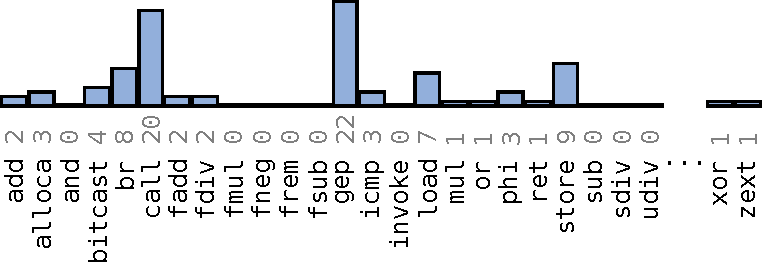
\includegraphics[width=0.9\linewidth]{figs/fingerprint-example.pdf}
% \vspace{-2ex}
% \caption{Example of a fingerprint.
% It is a fixed-size vector of integers with the frequency of each opcode. }
%  \label{fig:fingerprint-example}
% \end{figure}

% Formally, the hash structure can be defined as:
% \[  H[s] = \{ B_1 \in F_1 : |B_1| = s \} \]
% where $F_1$ contains the set of all basic blocks from the first input function and $|B|$ denotes the size of a given basic block.
% Therefore, a given $B_2 \in F_2$ is paired with $B_m \in H[|B_2|]$ such that:
% % %\[  B_m \in H[|B_2|] \land d(B_m,B_2) = min\{d(B_1,B_2) : B_1 \in H[|B_2|\} \]
% \[  d(B_m,B_2) = min\{d(B_1,B_2) : B_1 \in H[|B_2|\} \]
% where $d(B_1,B_2)$ represents the distance between the fingerprints of the basic blocks $B_1$ and $B_2$.


%Since the fingerprint of basic blocks have fixed size, i.e., the number of instruction opcodes, the distance between two basic blocks can be computed in constant time.


%as well as inspired by the more restrictive technique proposed by von Koch~et~al.~\cite{edler14}.


%These suitable candidate blocks are identified using a search strategy similar to the one used when searching for function candidates.
%For a given basic block $B_{2,j}$ from Function 2, 
%Basic blocks are paired by minimizing the Manhattan distance between their fingerprints, in a greedy manner.
%\[
%  \operatorname*{argmin}_{B_2 \in F_2} \{ d_1(F(B_1), F(B_2)) \} 
%\]

% \begin{figure}[h]
% \centering
% 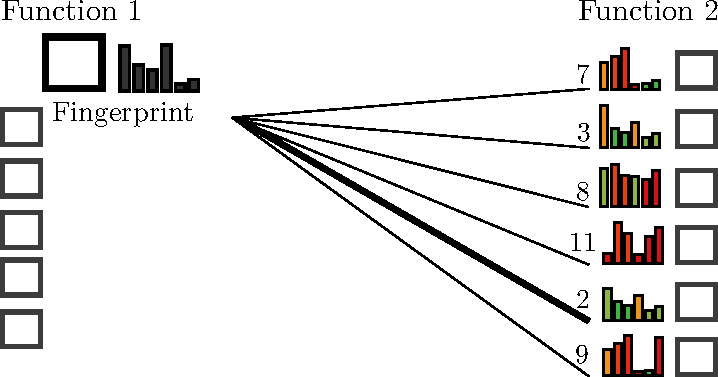
\includegraphics[width=0.8\linewidth]{figs/hyfm-ranking-full.pdf}
% \caption{Example illustrating one block from Function 2 being compared to all available blocks from Function 1. The pair with the smallest fingerprint distance will be considered for alignment.\fixme{PP: Not particularly informative imo.}}
%  \label{fig:hyfm-bb-pairing}
% \end{figure}

After pairing two basic blocks, $B_1$ and $B_2$, they have their instructions aligned (see Section~\ref{sec:bb-alignment}) and their merging profitability estimated (see Section~\ref{sec:multi-profitability}).
If they are deemed profitable, both blocks are removed from their respective working list.
Otherwise, only $B_1$ is removed from the working list of blocks from $F_1$, i.e., $B_2$ can still be paired with another block, but not $B_1$.
In other words, basic blocks from function $F_1$ are paired only once, even if its alignment is deemed unprofitable.
As a result, given two input functions, this pairing process is quadratic on their number of basic blocks.
This number is usually much smaller than the number of instructions in the function, so the cost of pairing is much lower than the cost of aligning whole functions in {\SOAName}, despite both being quadratic. For very large numbers of basic blocks, efficient nearest neighbor search techniques could keep the cost low but this was not needed in our experiments.

{\ProjName} pre-computes the fingerprint of every basic block in the input functions, which is a single linear cost over all their basic blocks and instructions.
Meanwhile, the distance between two fingerprints is computed in constant time, since the number of opcodes is a small constant.


% Note that the construction of the hash data structure is linear on the size of the functions $O(N)$ while the pairing itself can be quadratic on the number of basic blocks, $O(B^2)$.
% In the worst case, all basic blocks would have the same size and this exploration would be quadratic on the number of basic blocks.
% However, the number of basic blocks tend to be much smaller than the number of instructions and for large functions, basic blocks tend to vary in size.
% Therefore, it is unlikely that {\ProjName} will experience the worst case scenario for large functions.
% \textbf{TODO:} What is the average size of basic blocks per function (compare it with the average number of functions)? For functions with more than one basic block, how many of them have all basic blocks of the same size?

%%Given two functions, our goal is to produce a 


%To avoid breaking the semantics of the original program, we also need to maintain the order of the instructions for each of the functions.


%First, for one of the input functions, we group all its blocks by their number of instructions, except for the phi-nodes.
%We also pre-compute a fingerprint-based encoding of the basic blocks.
%This data structure allows us to quickly search for matching candidate blocks since they would have identical encodings.


%RestrictiveFM iterates over all blocks from the second input function, looking for a fully matching candidate block from the first function.

\subsection{Aligning Paired Basic Blocks}
\label{sec:bb-alignment}


%\subsubsection{\NW Alignment}
\label{sec:nw-alignment}

Basic blocks already represent a linearized sequence of instructions.
Any sequence alignment algorithm can be used on them the same way they can be used on linearized functions. The globally optimal \NW~\cite{needleman70} used by {\SOAName} remains a good choice. It may be quadratic in both space and time on the length of the sequences but basic block sequences are usually much shorter than functions, making the cost of alignment lower than in previous approaches. 

%\subsubsection{Linear Pairwise Alignment}
\label{sec:pa-alignment}

Our observations in Section~\ref{sec:motivation}, though, indicate that a globally optimal algorithm might be an excessive solution. %overkill.
Profitable sequences tend to be highly similar, so aligning them is usually straightforward. Based on this insight, we implemented a linear alignment algorithm. Its assumption is that profitable pairs of blocks are almost identical in terms of opcodes differing only in a few individual cases. This translates into a pairwise alignment of same size basic blocks where only corresponding instructions in the two blocks can match. Figure~\ref{fig:hyfm-alignment} illustrates two examples of basic blocks aligned using our strategy.
It also includes the costs estimated by our profitability analysis, which we discuss in Section~\ref{sec:multi-profitability}.

%As an alternative to the quadratic alignment algorithm, we also propose a linear alignment solution.
%This solution restricts pairing only between basic block of the same size.
%This restriction allows for a pairwise alignment, where only corresponding instructions in the paired basic blocks can match.
%Figure~\ref{fig:hyfm-alignment} illustrates two examples of basic blocks aligned using our linear pairwise strategy.

\begin{figure}[h]
\centering
  \begin{subfigure}{\linewidth}
  \center
  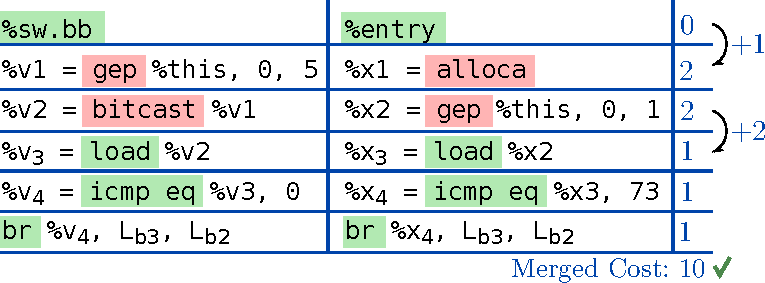
\includegraphics[width=0.6\linewidth]{src/lctes21/figs/hyfm-alignment-good.pdf}
  \caption{A profitable alignment. Both $OriginalCost$ and $MergedCost$ are 10. The final score is $OriginalCost - MergedCost = 0$.}
  \label{fig:hyfm-alignment-good}
  \end{subfigure}
\\
  \begin{subfigure}{\linewidth}
  \center
  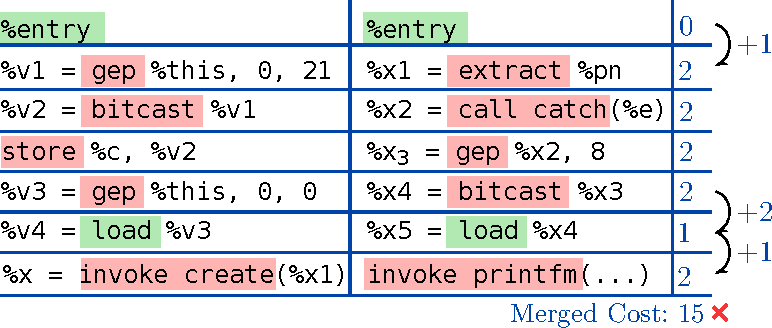
\includegraphics[width=0.6\linewidth]{src/lctes21/figs/hyfm-alignment-bad.pdf}
  \caption{An unprofitable alignment. $OriginalCost$ is 0 and $MergedCost$ is 15. The final score is $-3$. A negative score means it is unprofitable.}
  \label{fig:hyfm-alignment-bad}
  \end{subfigure}
\vspace{-2ex}
\caption{Two examples of the pairwise alignment. Only instructions in corresponding positions are aligned. Instructions match if they have the same opcode.}
 \label{fig:hyfm-alignment}
\end{figure}

Restricting alignment to basic blocks of the same size has the added benefit that it simplifies the pairing strategy. We only have to consider fingerprints for basic blocks of the same size, so we group them by block size and we restrict our search in the right group.
In the worst case, all basic blocks would have the same size and the search would remain quadratic on the number of basic blocks, as discussed in Section~\ref{sec:bb-rank}.
However, this is unlikely to happen in large functions, which is where the number of basic blocks might be a problem.
Overall, this solution is lean on memory usage and usually the fastest for aligning paired basic blocks, as corroborated by our evaluation in 
Section~\ref{sec:evaluation}.

\subsection{Multi-Tier Profitability Analysis}
\label{sec:multi-profitability}

{\ProjName} incorporates a multi-tier profitability analysis that enables it to bail out early from an unprofitable merge operation.
The first tier consists of a simple analysis applied on each pair of basic blocks selected for alignment, either accepting or rejecting the alignment between two blocks. 
The second tier consists of the same profitability analysis that is also performed by prior techniques, i.e., FMSA and {\SOAName}, which is responsible for evaluating whether the merged function is smaller than the original input functions.

The last column of Figure~\ref{fig:hyfm-alignment} shows how the first tier analysis is employed alongside the pairwise alignment strategy.
The same analysis can also be applied on pairs of basic blocks aligned using the \NW algorithm.
The analysis tries to estimate the cost of merging, the total number of instructions that will be necessary for merging the aligned blocks.
If two instructions match, then a single instruction is needed (i.e., a cost of \texttt{+1} is assigned to this entry).
If they mismatch, then both instructions are needed (i.e., a cost of \texttt{+2} is assigned to this entry).
Moreover, we need extra instructions to transition from matching subsequences to mismatching ones, and vice versa.
This is represented by the arrows in Figure~\ref{fig:hyfm-alignment}.
One branch instruction is needed to split control flow into two mismatching instructions, while two branch instructions are needed to join it back into a matching pair of instructions. 
The $MergedCost$ is the sum of all these costs.
The profitability score is defined as $OriginalCost - MergedCost$, where $OriginalCost$ is simply the number of instructions in the original basic blocks.
Therefore, a negative profitability score means that merging those two basic blocks is unprofitable. When this is the case, we ignore the alignment.

By rejecting individual basic block alignments, we are able to decide early whether merging a pair of functions might be profitable. If we rejected all block alignments, then by definition there is no point in merging the functions. Previous approaches, without a first tier analysis, have to rely on the second tier exclusively which is applied after the functions are merged.

\subsection{Independence from Code Layout}
%\fixme{MC: Is Code Reordering the right title here? As I understand it, this strength is basically because of the "consider all other blocks" aspect of the algorithm, so their source ordering becomes irrelevant. The insight is that we have decoupled the blocks from their position in the control flow. "Code Reordering" sounds like some more proactive smartness considering possible reordering, and a reader may expect to see this?  Maybe something like "Independence from Code Ordering" or some other phrase which captures this?}
Unlike all prior techniques, {\ProjName} is able to merge similar basic blocks regardless of their position in the control-flow graphs from the input functions.
Figure~\ref{fig:reordering-example} shows an example of  two functions that all prior techniques fail to merge even though they are highly similar. 

\begin{figure}[h]
  \centering
  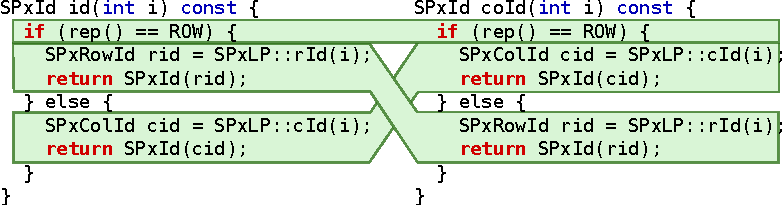
\includegraphics[width=0.95\linewidth]{src/lctes21/figs/soplex-example-one-column.pdf}
  \caption{Example with code reordering extracted from the \texttt{450.soplex} program.}
  \label{fig:reordering-example}
\end{figure}

% \begin{figure*}[t]
%   \centering
%   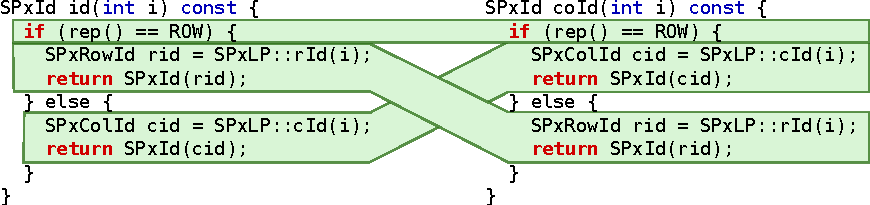
\includegraphics[width=0.75\textwidth]{figs/soplex-example.pdf}
%   \caption{Example with code reordering extracted from the \texttt{450.soplex} program.}
%   \label{fig:reordering-example}
% \end{figure*}

Due to their rigid linearization strategy, both FMSA and {\SOAName} are unable to properly match the basic blocks of the if-else structure, resulting in sub-optimal merged functions that are deemed unprofitable.
Their linearization traverses the control-flow graph in a canonical manner, preventing blocks from being rearranged for a better merging~\cite{rocha19,rocha20}.
Meanwhile, earlier techniques fail to merge this example as they are restricted to functions with identical control-flow graphs where corresponding blocks are merged~\cite{livska14,edler14,llvm-fm}.

{\ProjName} is able to correctly pair these basic blocks.
Because the basic blocks are rearranged, the label operands of the conditional branch need to be handled in order to preserve the program semantics.
For swapped label operands, {\ProjName} simply uses the optimized operand resolution proposed by {\SOAName}, where an \texttt{xor} operation is applied on the condition of the branch and the function identifier~\cite{rocha20}.



\section{Evaluation}
\label{sec:evaluation}

In this section, we compare {\ProjName} against {\SOAName}, presented in Chapter~\ref{chp:pldi20}.
First, we evaluate the code size reduction achieved by each technique, demonstrating that our approach is on a par with {\SOAName}. Then we show that {\ProjName} reduces significantly the overhead of function merging. % to such a degree that it becomes negligible.
Combined with the speedup in later stages of the compilation pipeline due to the reduced amount of code, {\ProjName} leads to faster end-to-end compilation than a baseline with no function merging enabled. Finally, we demonstrate how our contributions reduce the memory usage by several orders of magnitude. 

\subsection{Experimental Setup}
%We compare {\ProjName}, our novel function merging technique, against {\SOAName}, the  state-of-the-art~\cite{rocha20}.
In addition to evaluating \SOAName, we also consider four variations of our technique based on two dimensions:
1) the linear Pairwise Alignment (PA) versus the quadratic {\NW} Alignment (NW), both on a per basic block manner and
2) using a multi-tier profitability analysis versus using only the standard profitability analysis from {\SOAName}, which is the analysis applied on the whole function after generating the merged function.
As described in Section~\ref{sec:contribution}, the [PA] variant is, by construction, limited to merging only basic blocks of the same size. The [NW] variant can merge blocks of different sizes. The four variations are:

\begin{itemize}
    \item {[PA]}: PA with the Multi-tier Profitability analysis.
    \item {[PA,NMP]}: PA with No Multi-tier Profitability.
    \item {[NW]}: NW with the Multi-tier Profitability.
    \item {[NW,NMP]}: NW with No Multi-tier Profitability.
    %\item {[NW,SS]}: NW with Block Profitability but applied on blocks of the Same Size (SS).
\end{itemize}

%For \SOAName, we used the version published in their evaluation artifact~\cite{SalSSA}.
To keep the comparison fair, we implemented {\ProjName} for the same compiler as \SOAName, LLVM \fixme{v11}. We evaluated all techniques on the C/C++ programs from the SPEC CPU 2006 and the SPEC CPU 2017 benchmark suites~\cite{spec}. The baseline in all cases is the LLVM build in full LTO mode without any function merging.

We target the Intel x86 architecture.
All experiments were performed on a dedicated server with a quad-core Intel Xeon CPU E5-2650, 64 GiB of RAM, running Ubuntu 18.04.3 LTS. To minimize the effect of measurement noise, we repeated all compilation and runtime overhead experiments 5 times. We report the average values and their 95\% confidence intervals.

We evaluate all approaches in terms of code size reduction, time overhead of function merging, end-to-end compilation time, and peak memory usage. To better examine the trade-off between code size reduction and compilation time, we also introduce and measure a new metric called \textit{average reduction speed} which shows the efficiency of the optimization at reducing code size. This metric offers a single number that allows us to compare how different versions address the trade-off between compilation time and code size reduction.

\begin{definition}[Average Reduction Speed]
For a given input program and optimization, let $S$ and $S_0$ be the size of the program with and without the given optimization, respectively.
$R = S_0 - S$ represents the reduction achieved by such optimization.
Let $T$ be the running time of the optimization pass.
We define the \textit{average reduction speed} as:
\[
   ARS = \frac{R}{T}
\]  
\end{definition}

\subsection{Code Size Reduction} \label{sec:eval:size}

Figures~\ref{fig:size-reduction-both} reports the reduction on the size of the linked object files produced by the compiler.
While limiting alignment at a basic block granularity seems restrictive, its effect on code size is small. Even the worst performing variants of {\ProjName} are still within 3 percentage points of {\SOAName}, while both [PA] and [NW] achieve good results that are on a par with {\SOAName}. [PA]'s code size reduction varies from 5 percentage points worse to over 10 points better than {\SOAName}. On average, it is within 1 percentage point of the reduction achieved by {\SOAName}. [NW] almost always achieves better code size reduction than [PA] and on average outperforms {\SOAName} by a small margin. Since our primary aim is to reduce the high compile-time overheads of {\SOAName}
%, in the following sections,
a small loss of code reduction is acceptable. 

 \begin{figure}[h]
   \centering
 \begin{subfigure}{\textwidth}
 \center
   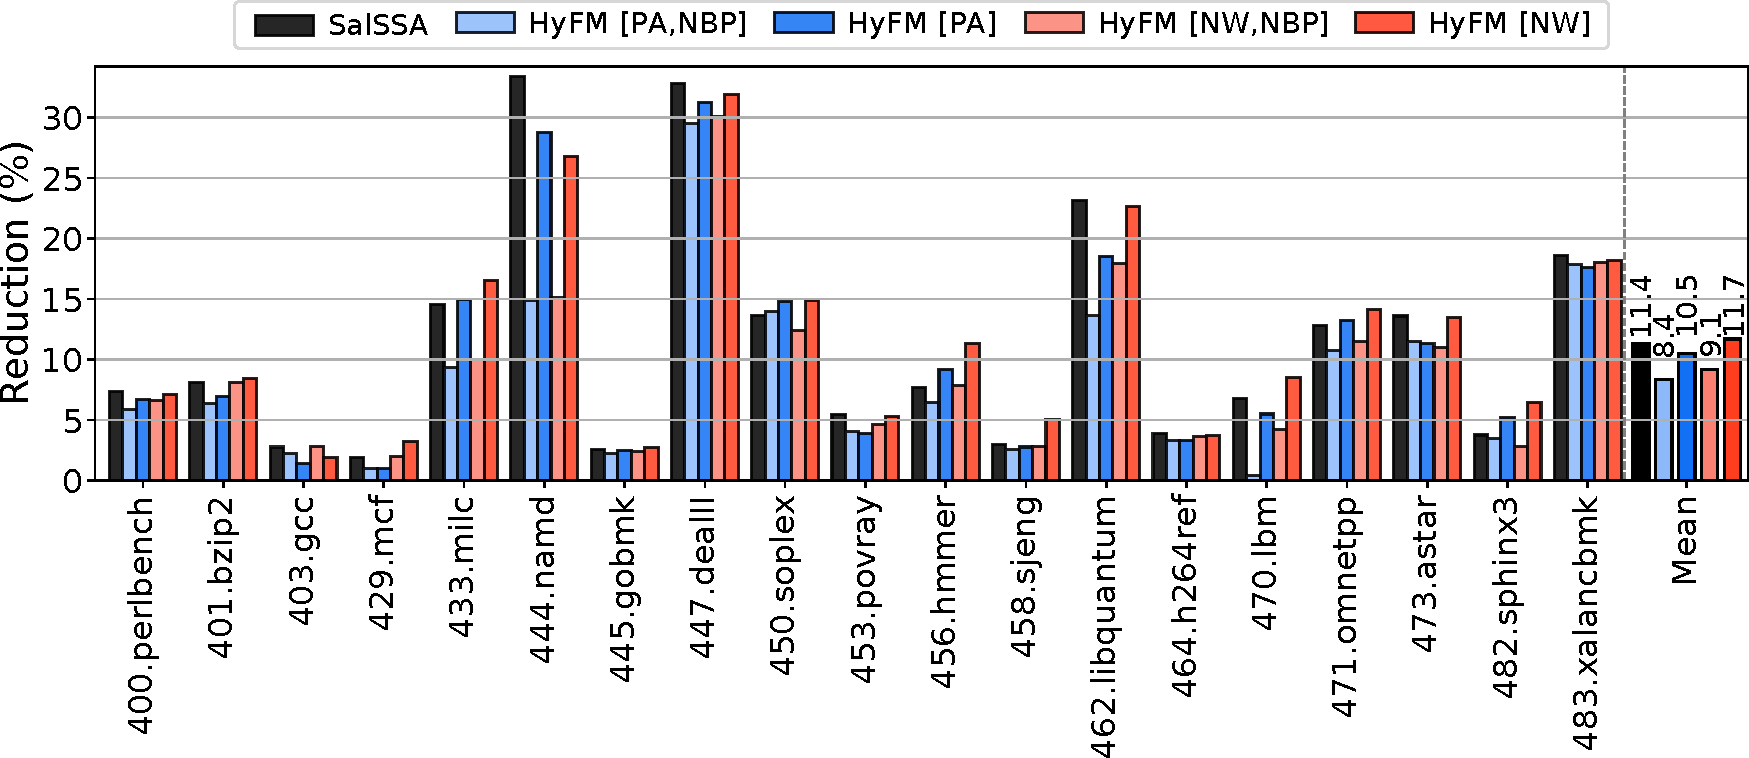
\includegraphics[width=\textwidth]{src/lctes21/figs/reduction-spec06.pdf}
 \caption{SPEC CPU 2006.}
 \label{fig:size-reduction-spec06}
 \end{subfigure}
 \\
 \begin{subfigure}{\textwidth}
 \center
   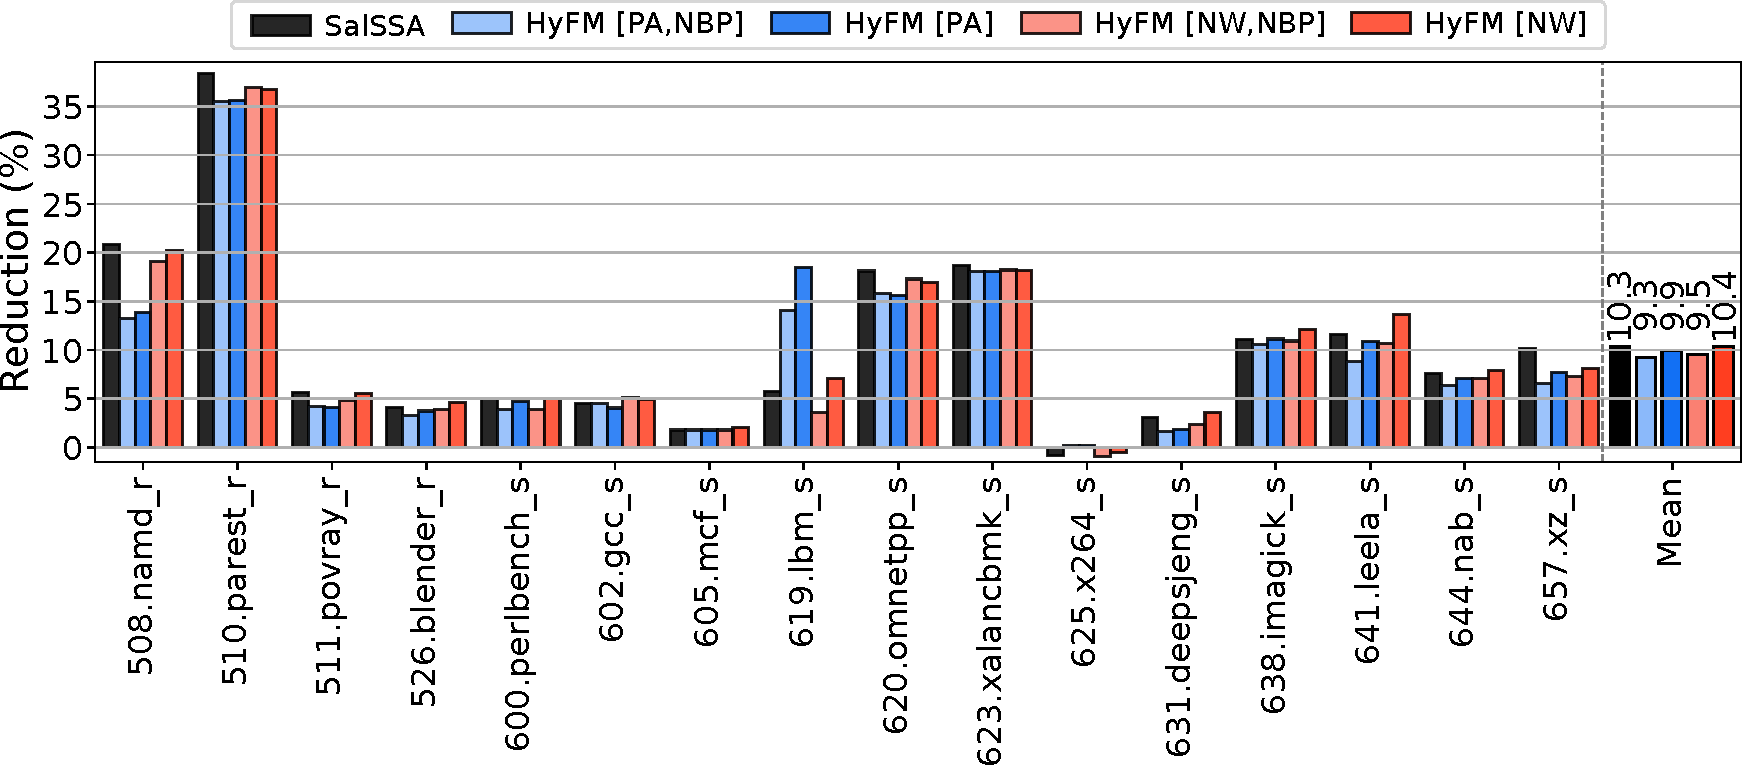
\includegraphics[width=\textwidth]{src/lctes21/figs/reduction-spec17.pdf}
 \caption{SPEC CPU 2017.}
 \label{fig:size-reduction-spec17}
 \end{subfigure}
 \caption{Linked object size reduction over LLVM LTO
      when performing function merging with {\ProjName} or {\SOAName} on SPEC CPU 2006 and 2017. On average, {\ProjName} improves code size reduction.}
  \label{fig:size-reduction-both}
 \end{figure}

%\begin{figure*}[t]
%  \centering
%  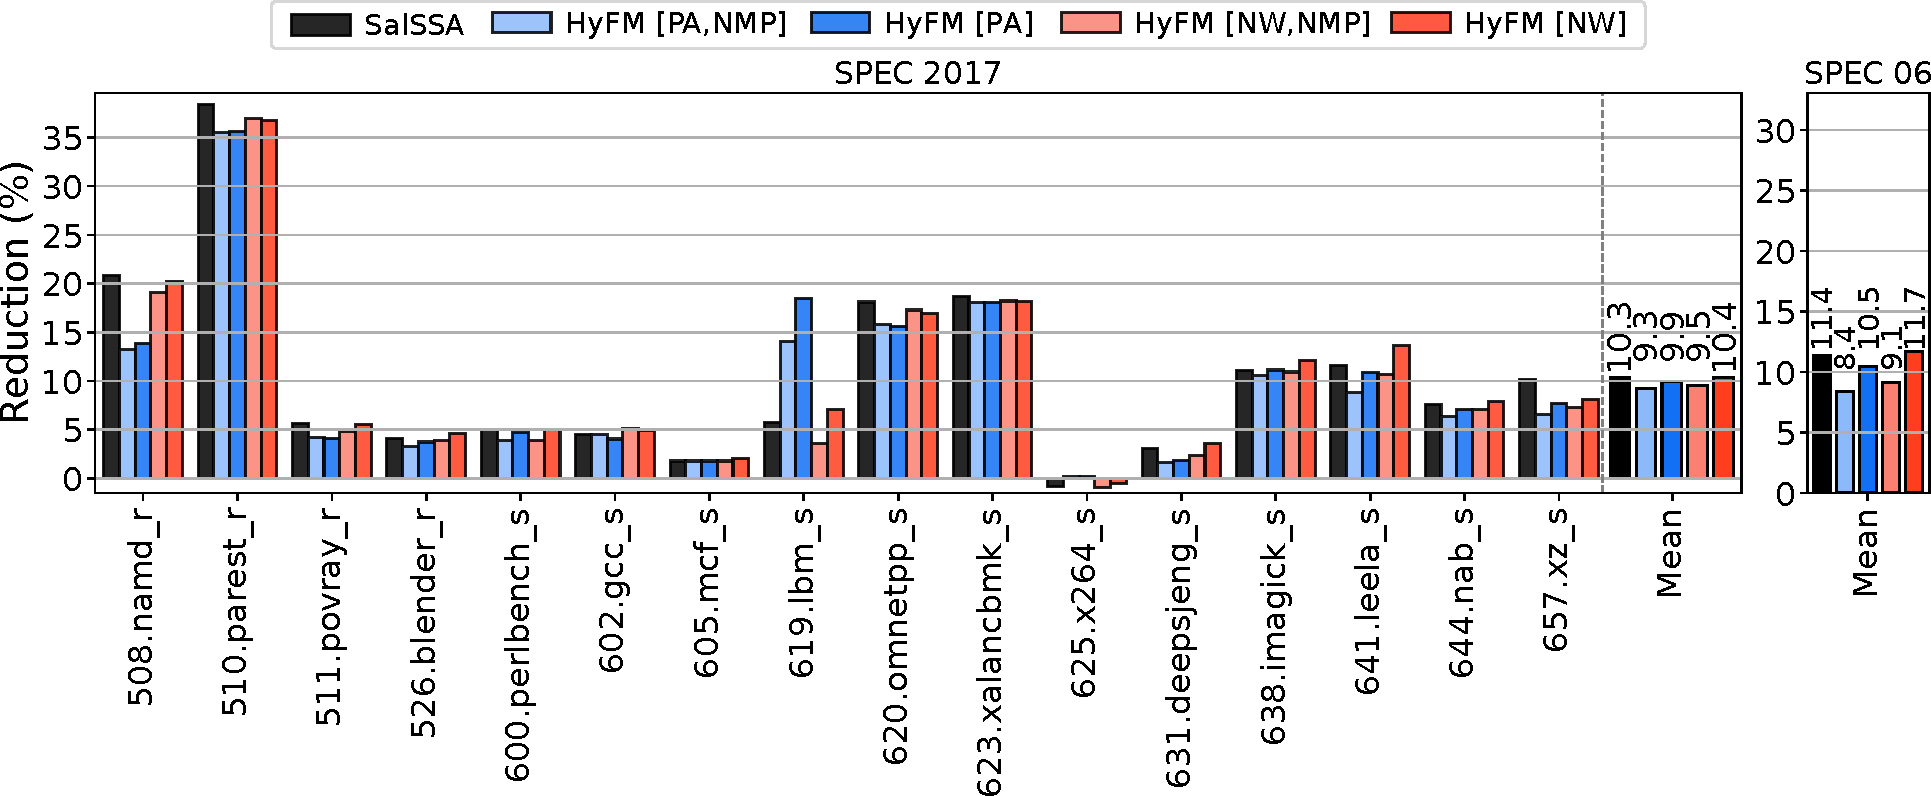
\includegraphics[width=0.95\linewidth]{src/lctes21/figs/reduction-spec17-06.pdf}
%  \caption{Linked object size reduction over LLVM LTO
%      when performing function merging with {\ProjName} or {\SOAName} on SPEC CPU 2006 and 2017. On average, {\ProjName} improves code size reduction.}
%  \label{fig:size-reduction-both}
%\end{figure*}

%Overall, {\ProjName} is on a par with the state of the art {\SOAName}.
%Since our primary aim is to reduce the high compile-time overheads of function merging, as described in Sections~\ref{sec:eval:compilation-time} and \ref{sec:eval:memory}, a small loss of code size reduction is acceptable.

%Even though restricting merging exclusively to basic blocks of the same size seems, at first glance, excessively strong, its effect on code size reduction is limited. On average, same size blocks lead to less than 1\% change compared to the state of the art.

These results indicate that the multi-tier profitability analysis is the single most important component of our approach. 
The two variants without the multi-tier profitability analysis, [PA,NMP] and [NW,NMP], are consistently worse than their counterparts that include this analysis, i.e. [PA] and [NW]. The multi-tier analysis contributes on average about 1 percentage point in code reduction for SPEC 2017 and more than 2 points for SPEC 2006.
The multi-tier profitability analysis has an important impact in the quality of the merged function.
While {\SOAName} lets unprofitable merged subsequences through as long as they are outweighed by profitable subsequences elsewhere in the merged function, {\ProjName} filters such unprofitable subsequences out.

The next most important effect comes from the choice of alignment algorithm. {\NW} is on average half a percentage point better than Pairwise Alignment for SPEC 2017 and about one percentage point better for SPEC 2006. Given that Pairwise Alignment only aligns blocks of the same size and does not try to discover optimal alignments, this difference is smaller than one would expect.
It indicates that profitable pairs of basic blocks tend to be extremely similar if not identical, as discussed in Section~\ref{sec:motivation}.
Still, {\NW} results in more size reduction.
When code size reduction is paramount, [NW] might be a better choice than [PA], but as we will see in Sections~\ref{sec:eval:compilation-time} and \ref{sec:eval:memory}, there is still a trade-off to navigate.

We get the biggest improvement by {[PA]} compared to {\SOAName} and {[NW]} for \texttt{lbm}, where it reduces the program's object file by 18.5\%, almost 13 percentage points more than the competition.
%%%%%%It's actually merging a few profitable basic blocks while giving up on several unprofitable merge sequences
%This comes from discovering a merging opportunity between two large basic blocks of the same size.
%Both {[PA]} and {[PA,NMP]} try merging these blocks but {\SOAName}, {[NW]}, and {[NW,NMP]} choose to focus on other candidates. Compared to {[PA,NMP]}, {[PA]} also finds and profitably merges the same function as {\SOAName} leading to even higher code size reduction.
{\SOAName} is able to profitably merge two pairs of functions.
On the other hand, {[PA,NMP]} chooses to perform a chained merge of the three largest functions in \texttt{lbm}, resulting in a significantly smaller binary.
This is possible because {[PA,NMP]} is merging some nearly identical pairs of basic blocks of the same size.
With the multi-tier profitability analysis, {[PA]} successfully identifies all four cases. 
{[NW]} fails to identify all of these cases, even though it is still better than {\SOAName}.
This exposes existing limitations in the cost model used by our profitability analysis.
%\fixme{Is this a cost model problem?}

The two worst results for {[PA]} are for the \texttt{namd} benchmark in both SPEC 2006 and SPEC 2017. {\SOAName} achieves close to 7 percentage points more than {[PA]} in code size reduction.
In both cases, Pairwise Alignment limits the number of successful merge operations. The variants using {\NW} recover most of the lost reduction. 

% \begin{figure}[h]
%   \centering
%   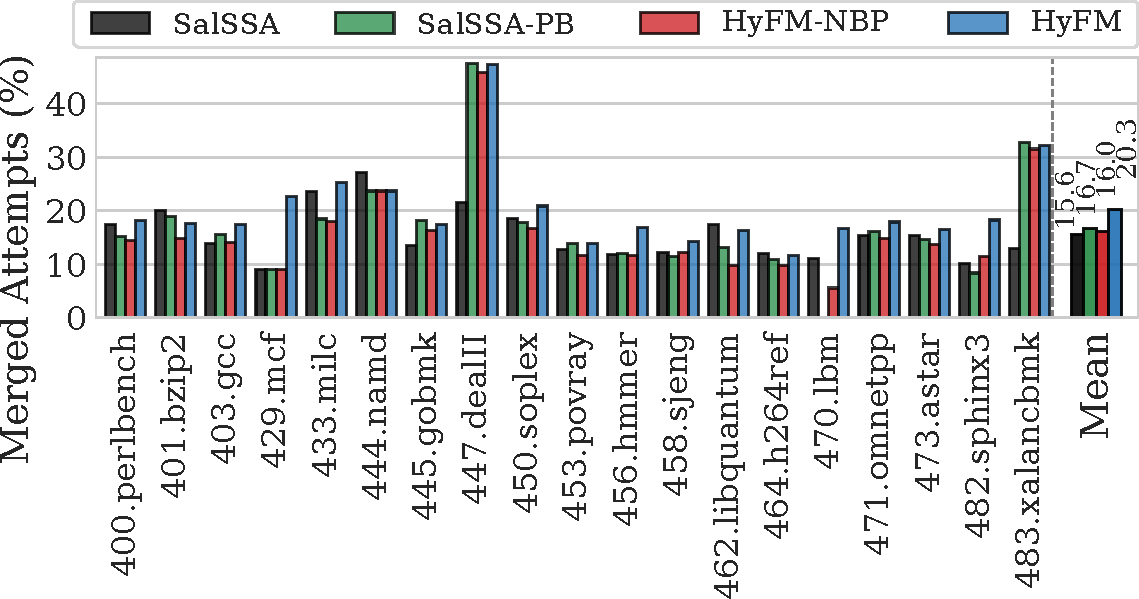
\includegraphics[width=\linewidth]{figs/merged-attempts-perc-spec06.pdf}
%   \caption{Number successful merging attempts on SPEC 2006.}
%   \label{fig:merged-attempts-perc-spec06}
% \end{figure}

% \begin{figure}[h]
%   \centering
%   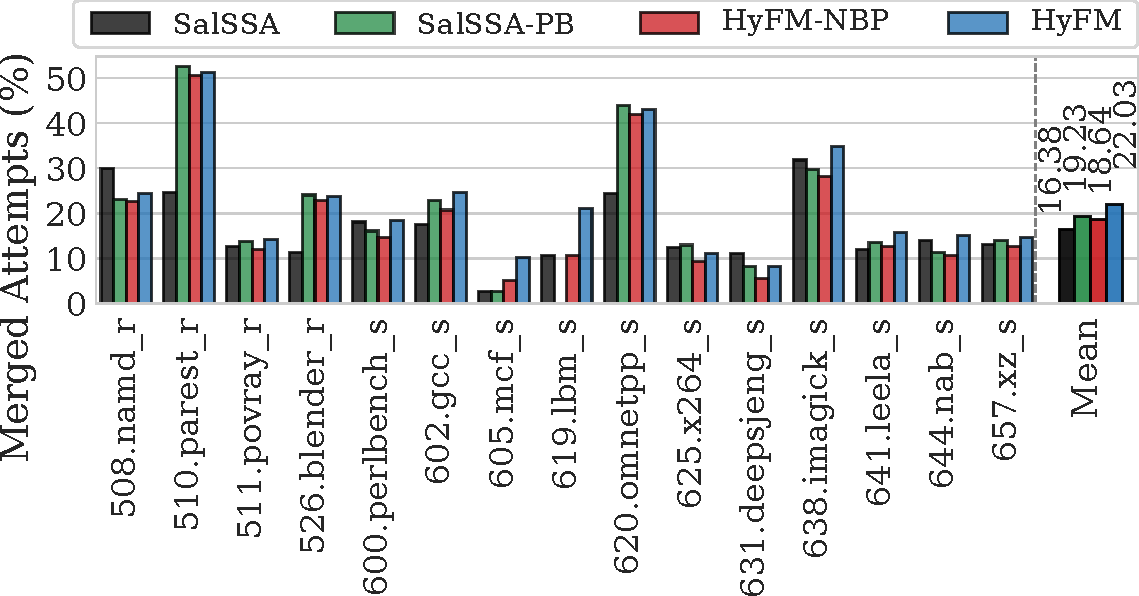
\includegraphics[width=\linewidth]{figs/merged-attempts-perc-spec17.pdf}
%   \caption{Number of successful merging attempts on SPEC 2017.}
%   \label{fig:merged-attempts-perc-spec17}
% \end{figure}

% \begin{figure}[h]
%   \centering
%   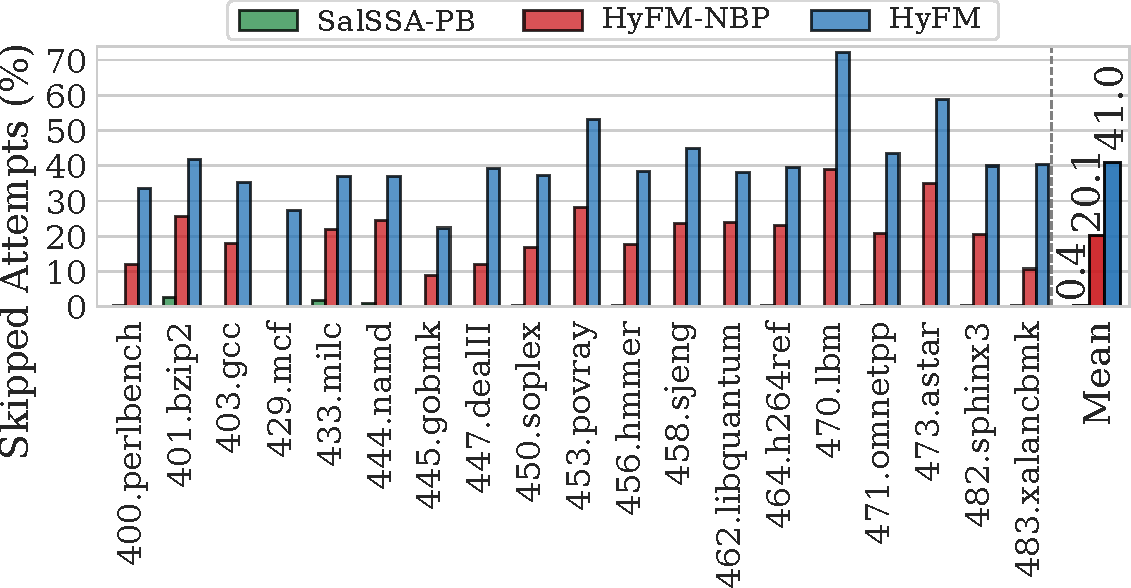
\includegraphics[width=\linewidth]{figs/skipped-attempts-perc-spec06.pdf}
%   \caption{Number of skipped merging attempts on SPEC 2006.}
%   \label{fig:skipped-attempts-perc-spec06}
% \end{figure}

% \begin{figure}[h]
%   \centering
%   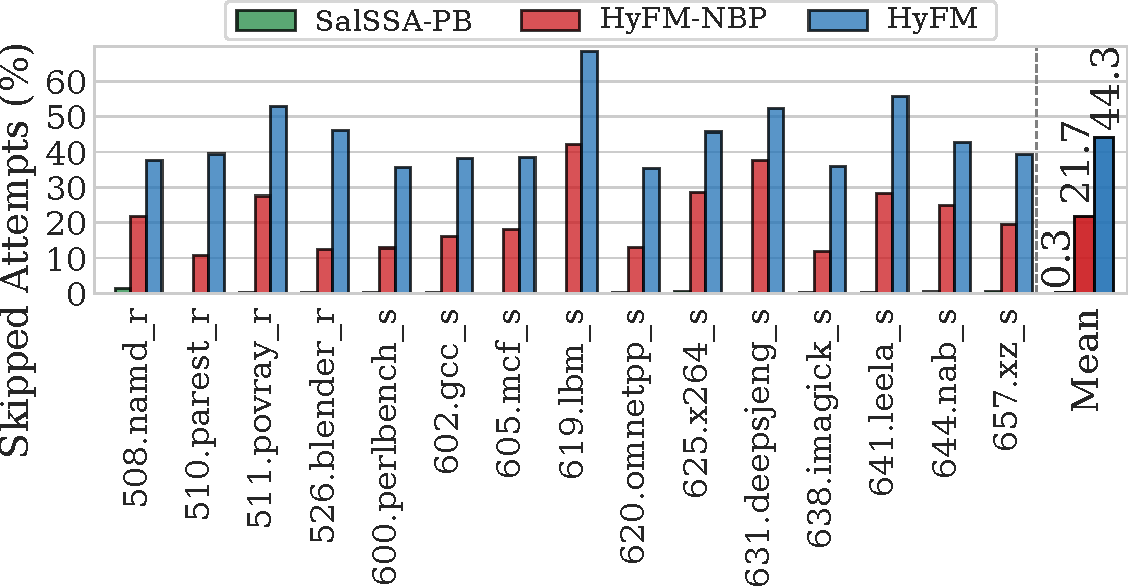
\includegraphics[width=\linewidth]{figs/skipped-attempts-perc-spec17.pdf}
%   \caption{Number of skipped merging attempts on SPEC 2017.}
%   \label{fig:skipped-attempts-perc-spec17}
% \end{figure}


% \begin{figure*}[h]
%   \centering
%   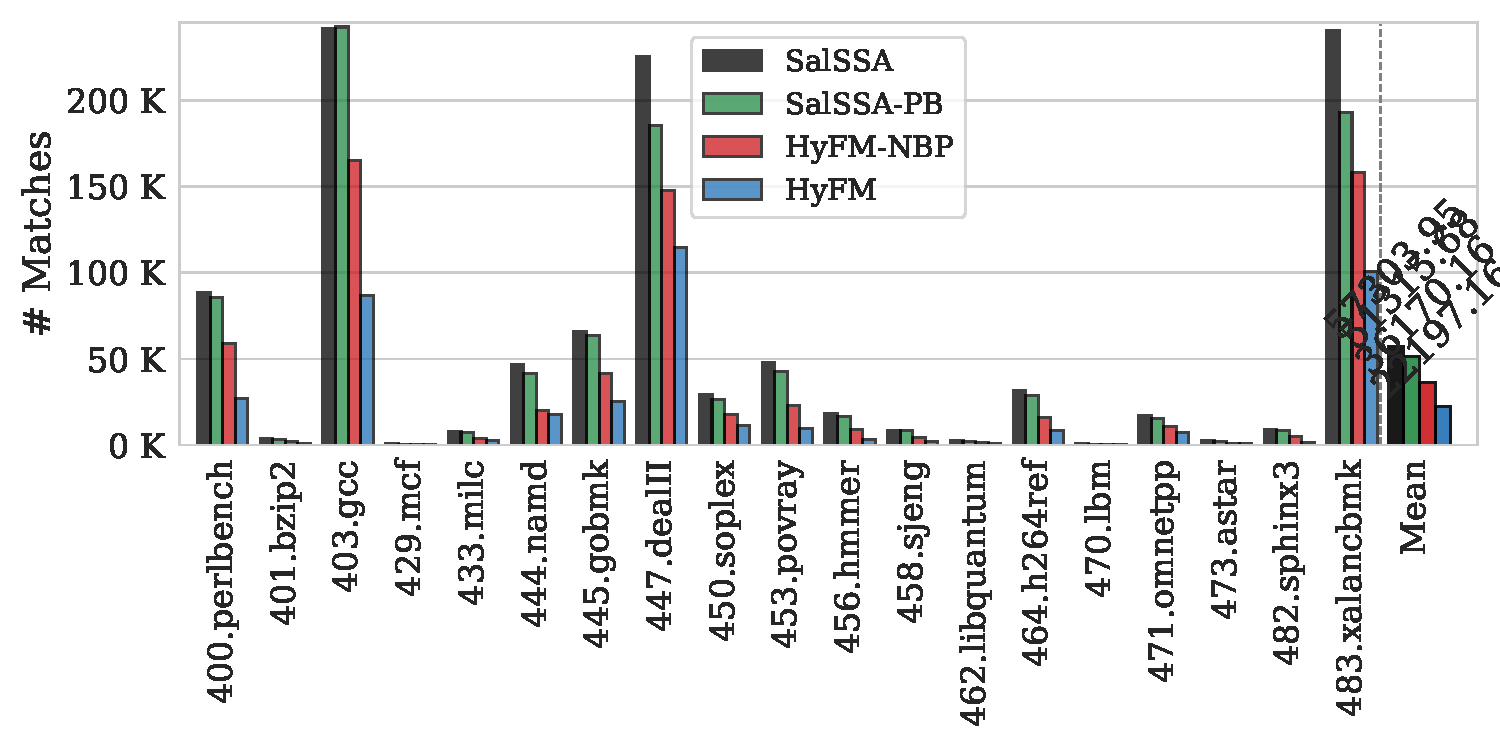
\includegraphics[width=0.85\linewidth]{figs/total-num-matches-spec06.pdf}
%   \caption{Total number of matching entries, including profitable and unprofitable attempts. SPEC 2006.}
%   \label{fig:total-num-matches-spec06}
% \end{figure*}

% \begin{figure*}[h]
%   \centering
%   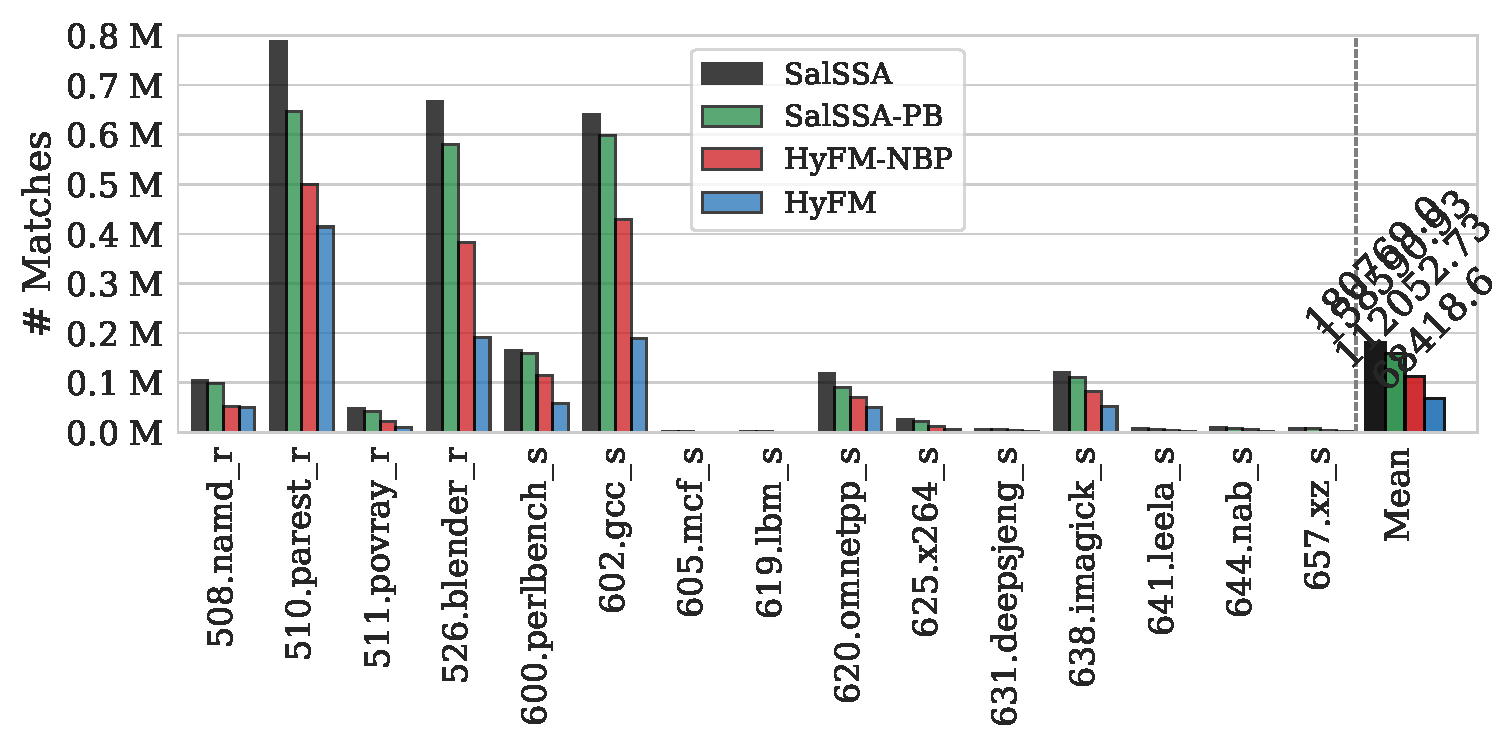
\includegraphics[width=0.85\linewidth]{figs/total-num-matches-spec17.pdf}
%   \caption{Total number of matching entries, including profitable and unprofitable attempts. SPEC 2017.}
%   \label{fig:total-num-matches-spec17}
% \end{figure*}

\subsection{Speeding Up Function Merging} \label{sec:eval:pass-speedup}

 \begin{figure}[h]
   \centering
 \begin{subfigure}{\textwidth}
 \center
   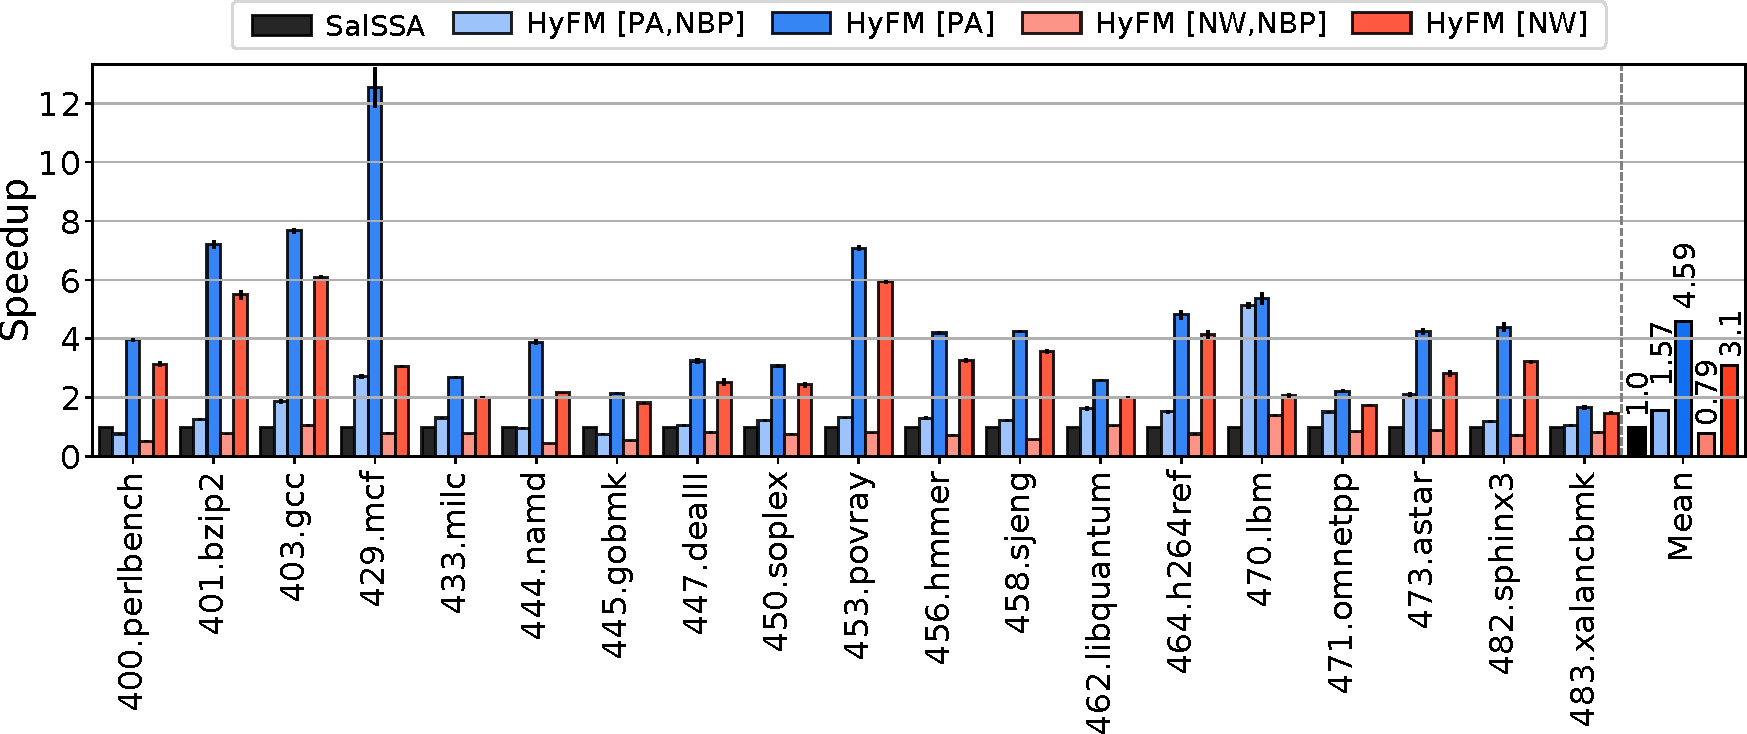
\includegraphics[width=\textwidth]{src/lctes21/figs/speedup-spec06.pdf}
 \caption{SPEC CPU 2006.}
 \label{fig:speedup-spec06}
 \end{subfigure}
 \\
 \begin{subfigure}{\textwidth}
 \center
   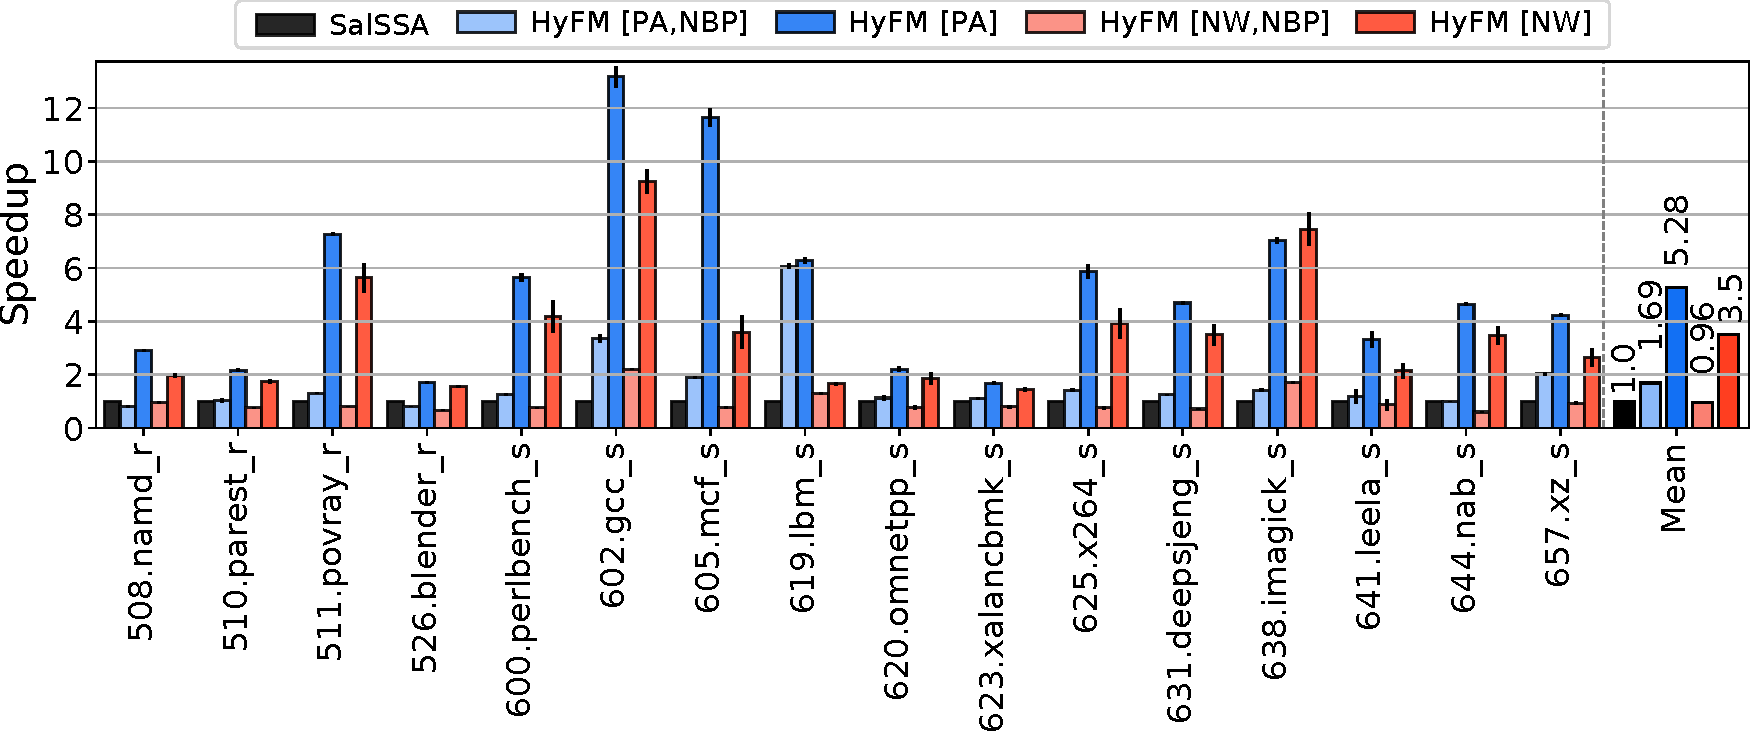
\includegraphics[width=\textwidth]{src/lctes21/figs/speedup-spec17.pdf}
 \caption{SPEC CPU 2017.}
 \label{fig:speedup-spec17}
 \end{subfigure}
 \caption{Speedup of the function merging pass in isolation relative to {\SOAName}. The multi-tier profitability analysis reduces the number of unprofitable merge operations leading to a significant speedup.}
  \label{fig:speedup-both}
 \end{figure}

%\begin{figure*}[t]
%  \centering
%  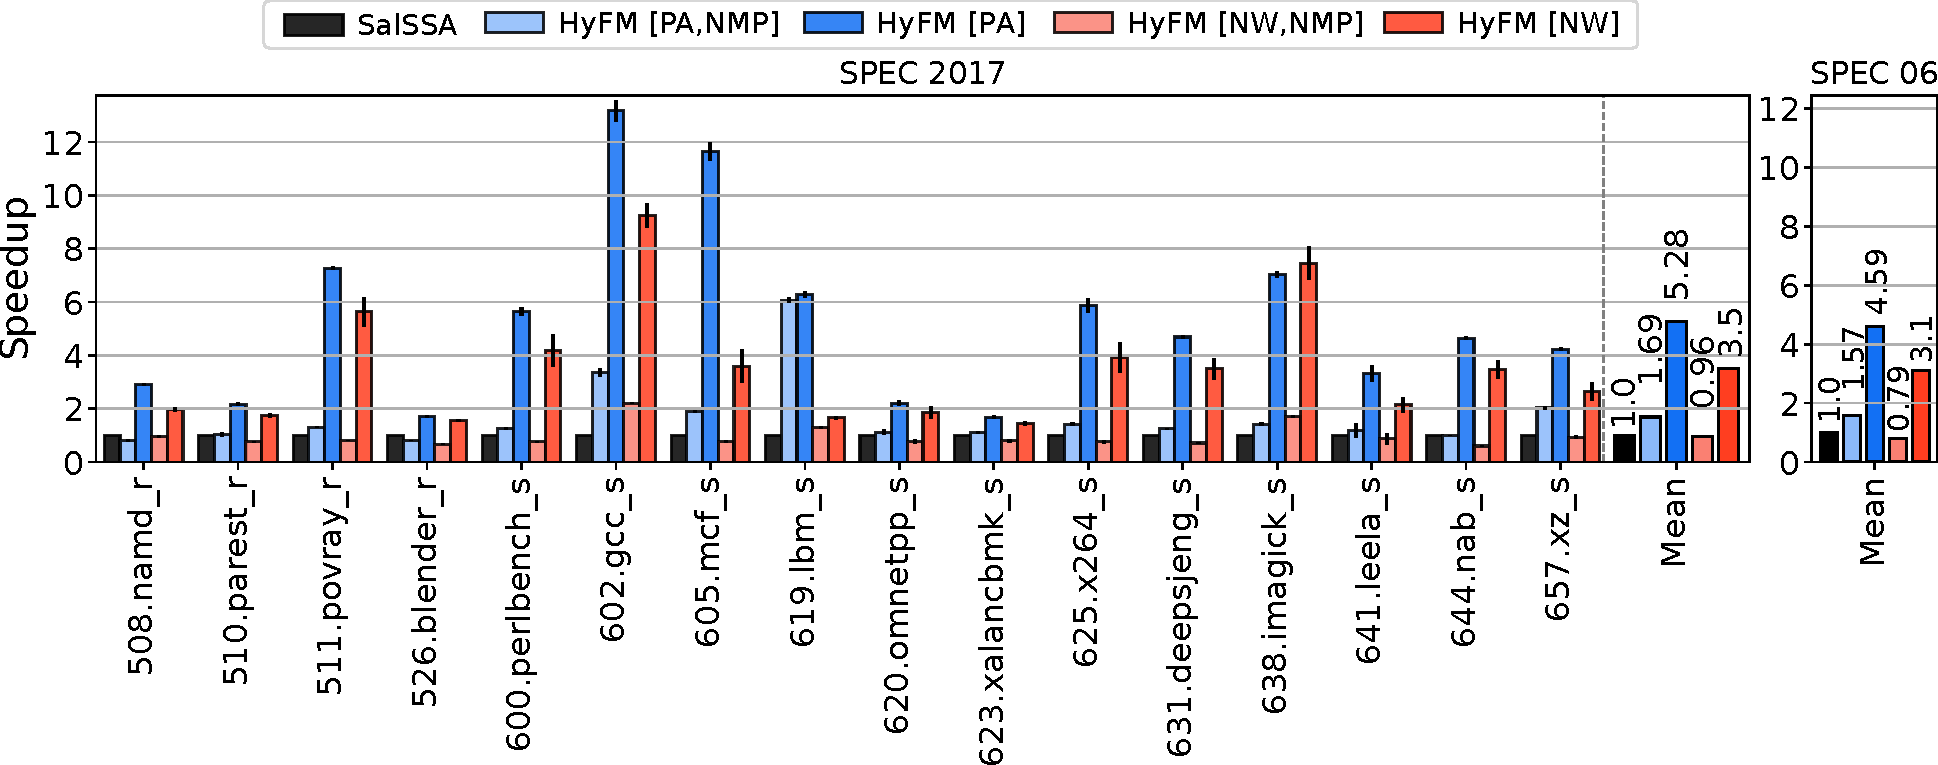
\includegraphics[width=0.95\linewidth]{src/lctes21/figs/speedup-spec17-06.pdf}
%  \caption{Speedup of the function merging pass in isolation relative to {\SOAName}. The multi-tier profitability analysis reduces the number of unprofitable merge operations leading to a significant speedup.}
%  \label{fig:speedup-both}
%\end{figure*}

Figure~\ref{fig:speedup-both} shows the speedup of {\ProjName} relative to {\SOAName}.
This considers only the time taken by the function merging pass, which include all stages discussed in Section~\ref{sec:motivation:breakdown}.
Our novel technique achieves an impressive speedup. For {[PA]} it is on average $5.28\times$ faster for SPEC 2017 and $4.59\times$ for SPEC 2006. Even in the worst case, it achieves a \fixme{50}\% speedup. In the best case, for the SPEC 2017 \texttt{gcc}, function merging under {\ProjName} takes a total of 23.5 seconds instead of 302, which translates to almost $13\times$ less time.

%The two variants with the multi-tier profitability analysis achieve on average three to four times higher speedups than their counterparts without it. This is a direct result of bailing out early. For most benchmarks, only a small number of candidate pairs is profitable. The majority are unprofitable but SalSSA has to merge them anyway to determine their profitability. This is expensive and wasteful. Our approach,on the other hand, is able to estimate profitability early. Only function pairs with any chance of being profitable, that is pairs with at least one profitable pair of basic blocks, move forward to the expensive merge stage.
%The linear pairwise alignment contributes to the performance improvement, too. The variants using pairwise alignment run on average 48% to 98% faster than their Needleman-Wunsch counterparts. The most pronounced case is for lbm where [PA] is around3×faster than [NW]. The blocks paired in lbm are longer than usual, so the quadratic Needleman-Wunsch spends significantly more time trying to align them than our linear pairwise algorithm. Figure 7 shows that the added pairing restrictions from [PA], to focus on blocks with higher similarities, also benefits later stages.
%All components of HyFM contribute towards this result but the multi-tier profitability analysis has the most significant impact. As we show in Figure 7, even though the time spent on the alignment strategy becomes negligible for both [PA,NMP] and [PA], the lack of a multi-tier profitability analysis may degrade the stages associated with code generation. If we accept the alignment for any pair of basic blocks, we may end up producing complex merged functions— code with an excessive amount of branches, phi-nodes,and operand selections — slowing down SSA reconstruction and code simplification. This effect can be observed with [PA,NMP] for many benchmarks in Figure 7. Most notably, for the blender benchmark, [PA,NMP] is slower than SalSSA due to its added pressure on the SSA reconstruction algorithm, even though its alignment strategy runs much faster. For this reason, enabling the multi-tier profitability analysis has a positive impact on later stages.

All components of {\ProjName} contribute towards this result but the multi-tier profitability analysis has the most significant impact. The two variants with the multi-tier profitability analysis achieve on average three to four times higher speedups than their counterparts without it.
To help us understand why, Figure~\ref{fig:breakdown-spec17} shows how the compilation time of each approach is distributed across its various stages. 
Even though the time spent on the alignment strategy becomes negligible with {\ProjName}, the less optimal alignment often produces complex merged functions --- code with an excessive amount of branches, phi-nodes, and operand selections --- slowing down SSA reconstruction and code simplification. This effect is very pronounced for the \texttt{blender} benchmark, where both [PA,NMP] and [NW,NMP] are slower than {\SOAName} due to the added pressure on the SSA reconstruction algorithm, even though the alignment overhead is practically zero.
Similar effects can be observed in other benchmarks.

\begin{figure}[h]
  \centering
  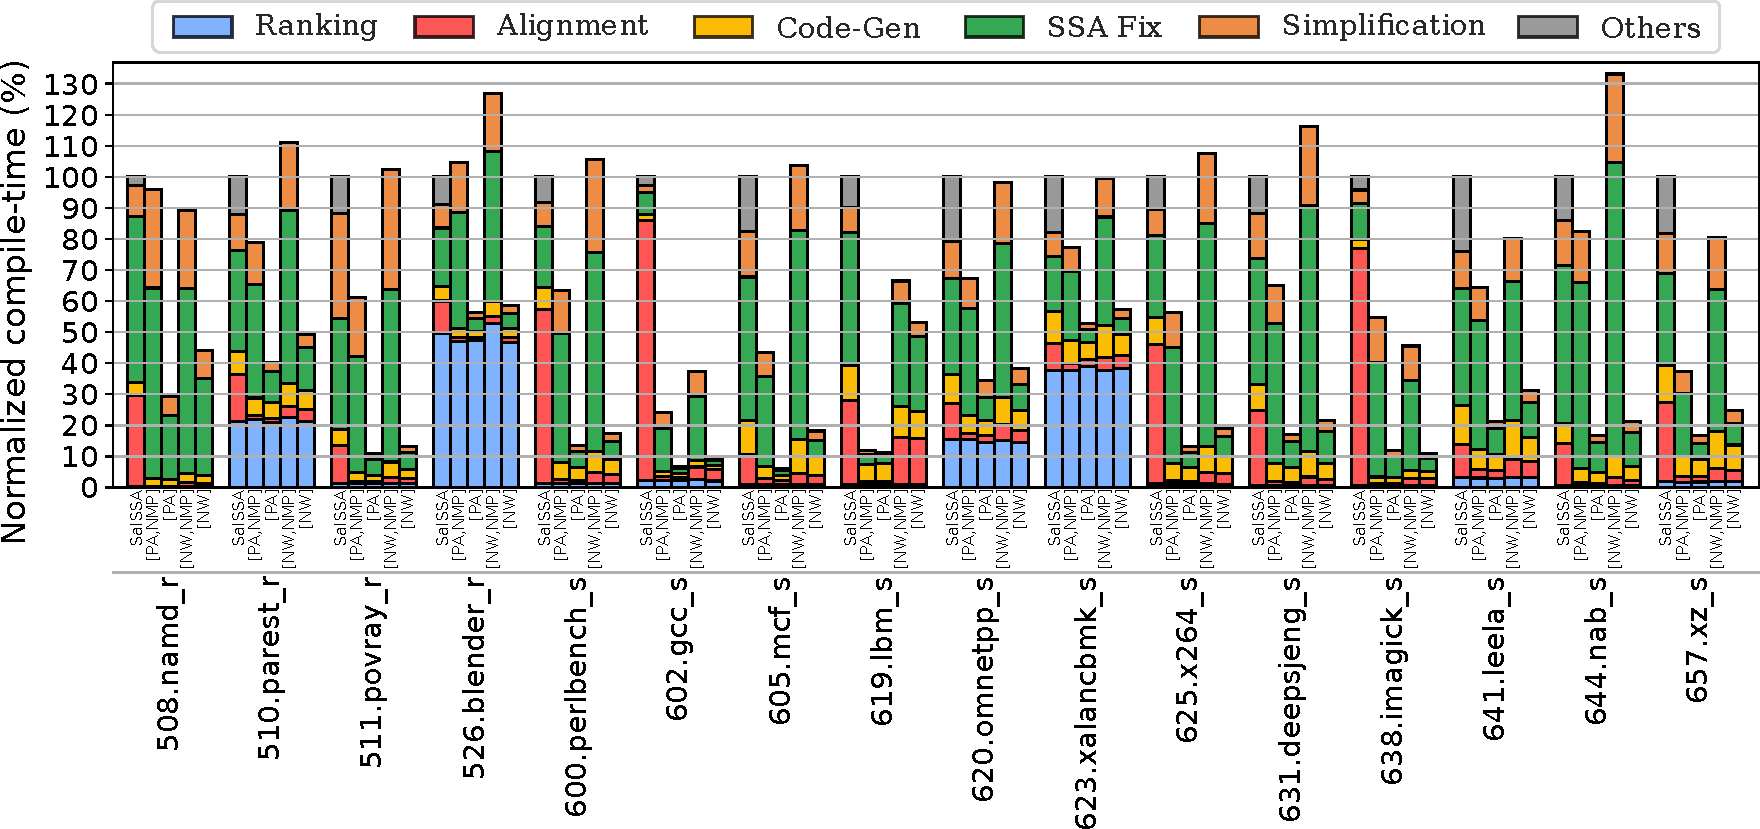
\includegraphics[width=\linewidth]{src/lctes21/figs/breakdown-full-spec17.pdf}
  \caption{Breakdown of the relative runtime for the different stages of the function merging pass. All measurements are normlized by \SOAName's total runtime on the corresponding benchmark. For every benchmark, we show {\SOAName}, [PA,NMP], [PA], [NW,NMP], and [NW], in this order. }
  \label{fig:breakdown-spec17}
\end{figure}

Enabling the multi-tier profitability analysis counters this effect by focusing code generation exclusively on profitable blocks and functions. Most of the complex basic blocks {\ProjName} generates are not profitable for the same reason it is expensive to process them. First-tier profitability filters them out. On top of that, most paired functions under either {\SOAName} or {\ProjName} are unprofitable. {\SOAName} has to merge them anyway to determine their profitability. This is expensive and wasteful. Our approach, on the other hand, is able to estimate profitability early. Only function pairs with any chance of being profitable, that is pairs with at least one profitable pair of basic blocks, move forward to the expensive merge stage.

The linear pairwise alignment contributes to the performance improvement, too. The variants using pairwise alignment run on average 48\% to 98\% faster than their {\NW} counterparts.
%The most pronounced case is for \texttt{mcf} where {[PA]} is approximately $3\times$ faster than {[NW]}. Candidate basic block pairs in \texttt{mcf} are longer than usual, so the quadratic {\NW} spends significantly more time trying to align them than our linear pairwise algorithm. 
The most pronounced case is for \texttt{lbm} where {[PA]} is around $3\times$ faster than {[NW]}. The blocks paired in \texttt{lbm} are longer than usual, so the quadratic {\NW} spends significantly more time trying to align them than our linear pairwise algorithm.
Figure~\ref{fig:breakdown-spec17} shows that the added pairing restrictions from [PA], to focus on blocks with higher similarities, also benefits later stages.

\subsection{End-to-End Compilation Time} \label{sec:eval:compilation-time}

We have also analyzed separately the end-to-end compilation time because reducing code size through function merging has knock-on effects in later stages of the compilation pipeline.
The first order effect is that reducing the number of functions tends to reduce compilation time.
This is not guaranteed though, because merged functions may be more complex, potentially slowing down later compiler analyses and transformations.
Moreover, the time spent merging functions may be so large that it negates any benefits from having fewer functions later in the pipeline.

Even though on a few occasions {\SOAName} reduces end-to-end compilation time, in general, its overhead is large enough to result in an overall compilation time slowdown, 9.5\% to 4.1\% for SPEC 2017 and 2006 respectively.
In contrast, {\ProjName} is so much faster that its compilation time overhead is matched or outweighed by the speedup in later stages. 
This reduction is marginal for SPEC 2017, but for SPEC 2006 {[PA]} reduces the average compilation time by 2.3\% and {[NW]} by 1.6\%.
There is only a single case where {[PA]} results in a significant end-to-end slowdown, 10\% for \texttt{blender}.
%While this is still an improvement compared to {\SOAName}, \fixme{EXPLAIN}.
Figure~\ref{fig:breakdown-spec17} shows that, although [PA] runs faster than {\SOAName}, both of them spent a significant amount of time ranking the function candidates, due to its large number of functions.
Ranking alone in this case takes around 70 seconds. %However, this is beyond the scope of this paper.

Overall, we believe that this reduction in end-to-end compilation time is a very important result. While {\ProjName} is still achieving code-size reduction on par with the state-of-the-art, it does not have the detrimental effects of {\SOAName} on the overall compilation process and can be safely applied.

 \begin{figure}[h]
   \centering
 \begin{subfigure}{\textwidth}
 \center
   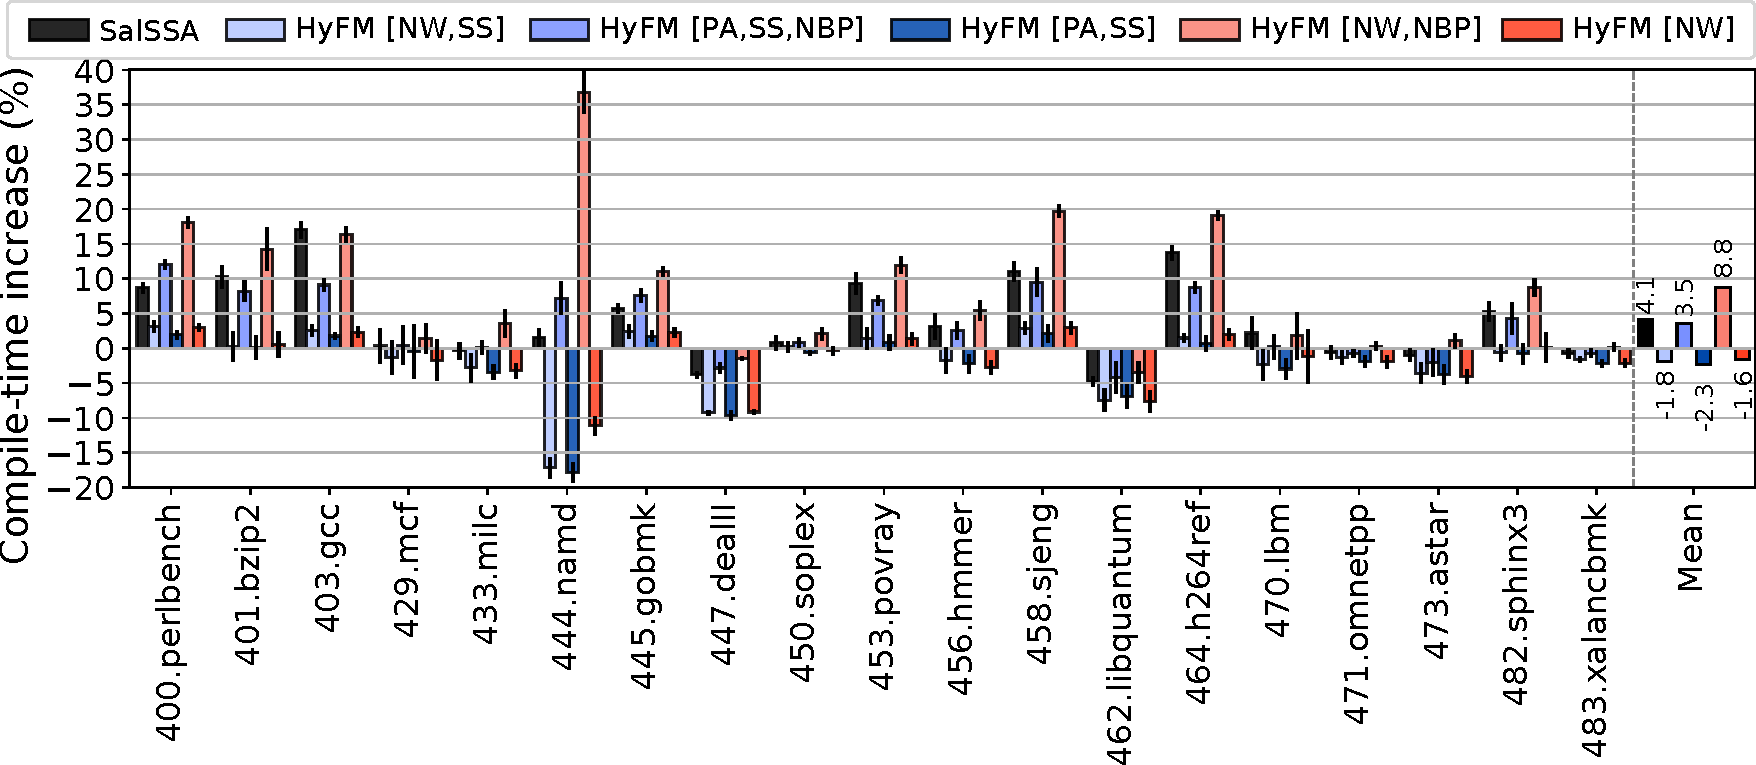
\includegraphics[width=\textwidth]{src/lctes21/figs/compiletime-spec06.pdf}
 \caption{SPEC CPU 2006.}
 \label{fig:compiletime-spec06}
 \end{subfigure}
 \\
 \begin{subfigure}{\textwidth}
 \center
   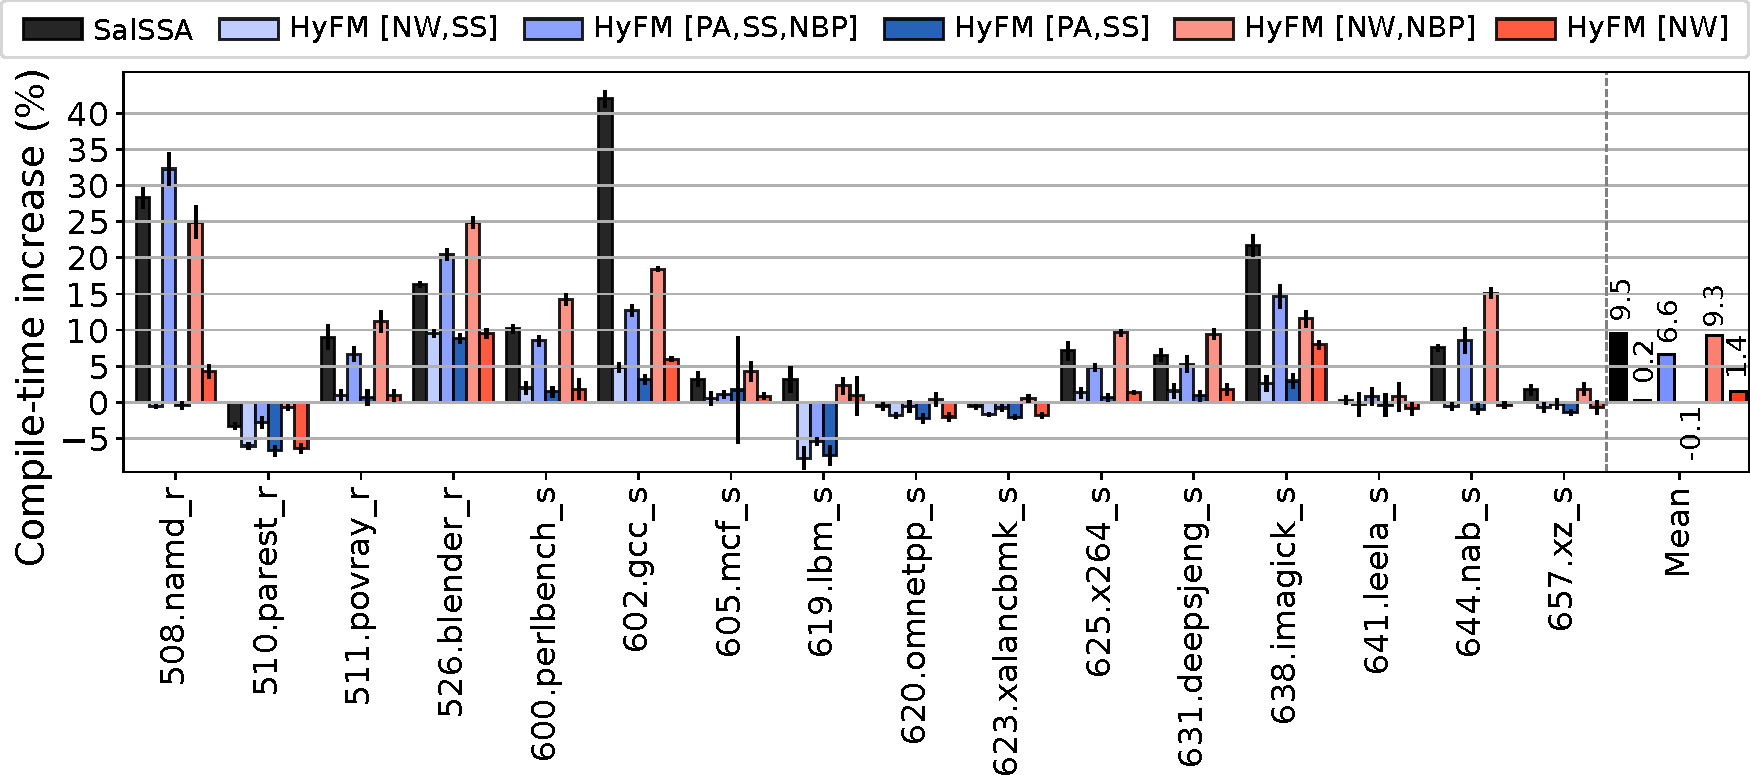
\includegraphics[width=\textwidth]{src/lctes21/figs/compiletime-spec17.pdf}
 \caption{SPEC CPU 2017.}
 \label{fig:compiletime-spec17}
 \end{subfigure}
 \caption{Normalized end-to-end compilation time for SPEC 2017 and SPEC 2006 relative to LLVM LTO.}
  \label{fig:compiletime-both}
 \end{figure}

%\begin{figure*}[h]
%  \centering
%  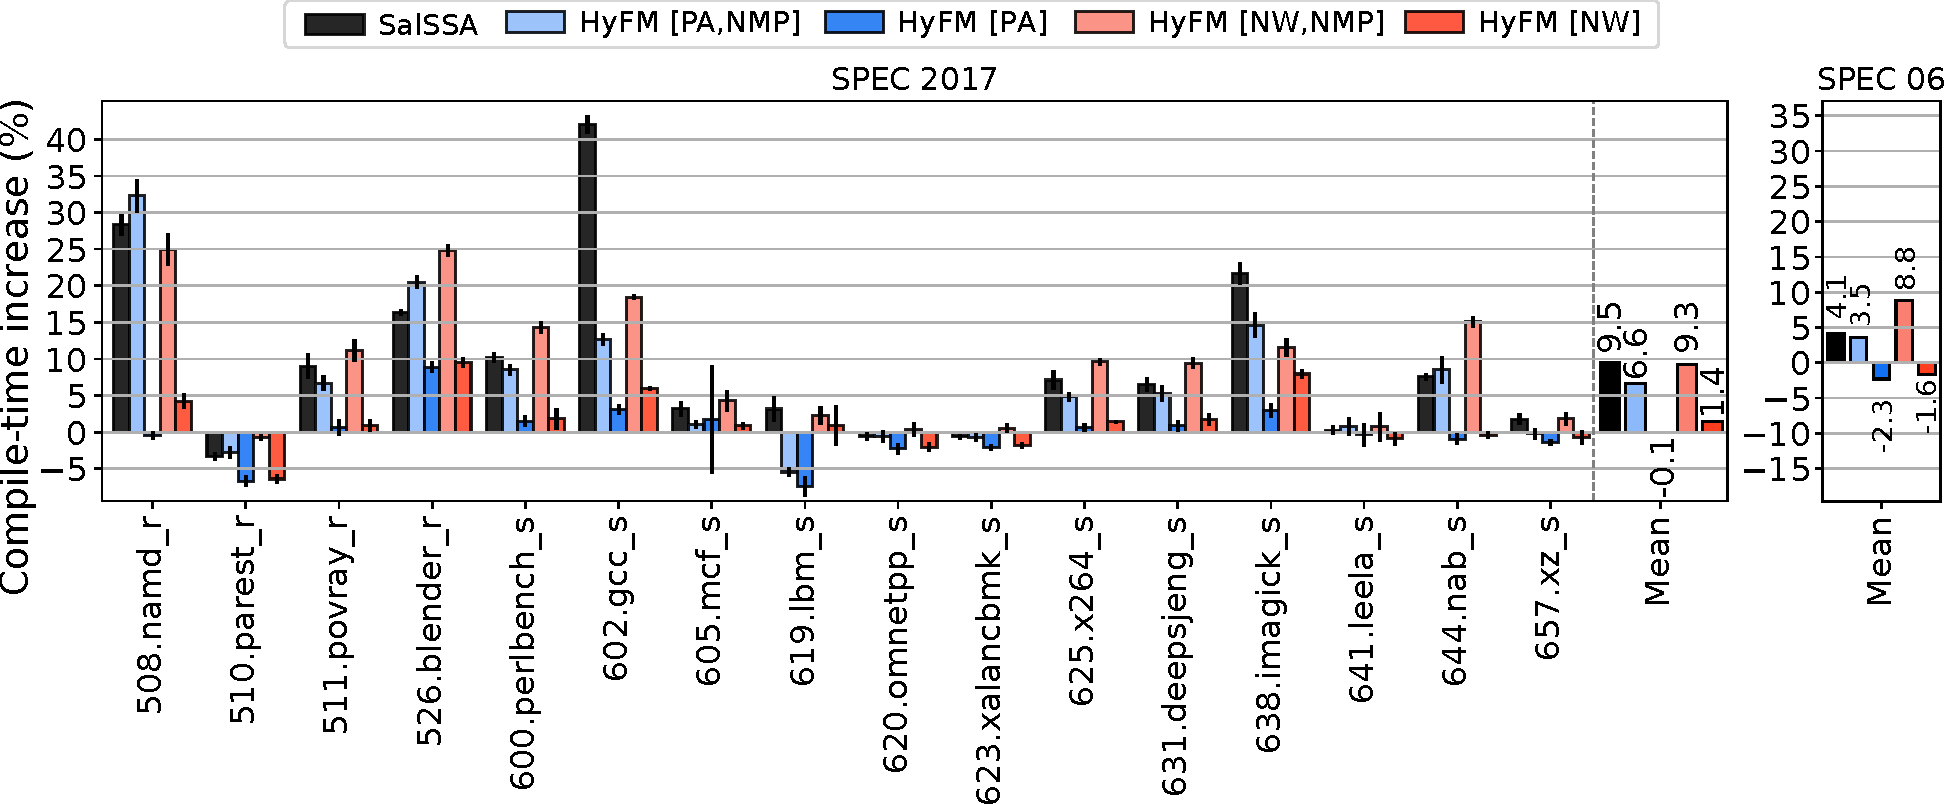
\includegraphics[width=0.95\linewidth]{src/lctes21/figs/compiletime-spec17-06.pdf}
%  \caption{Normalized end-to-end compilation time for SPEC 2017 and SPEC 2006 relative to LLVM LTO.}
%  \label{fig:compilation-both}
%\end{figure*}


\subsection{Code Size and Compilation Time Trade-Off} \label{sec:eval:trade-off}

While the multi-tier profitability analysis improves both code-size reduction and compilation speed, the choice of alignment algorithm introduces a trade-off. Pairwise alignment is better for speed, {\NW} is better for code-size reduction. 
In terms of compilation efficiency, i.e. how much code size reduction we get for the effort we put in, the picture is clearer. In Figure~\ref{fig:ars-both}, the \textit{average reduction speed} suggests that {[PA]} achieves the ideal trade-off, with an average reduction speed of 115.3~KB/s, which is around $3\times$ greater than {\SOAName}'s and 20\% to 40\% greater than [NW].


 \begin{figure}[h]
   \centering
 \begin{subfigure}{\textwidth}
 \center
   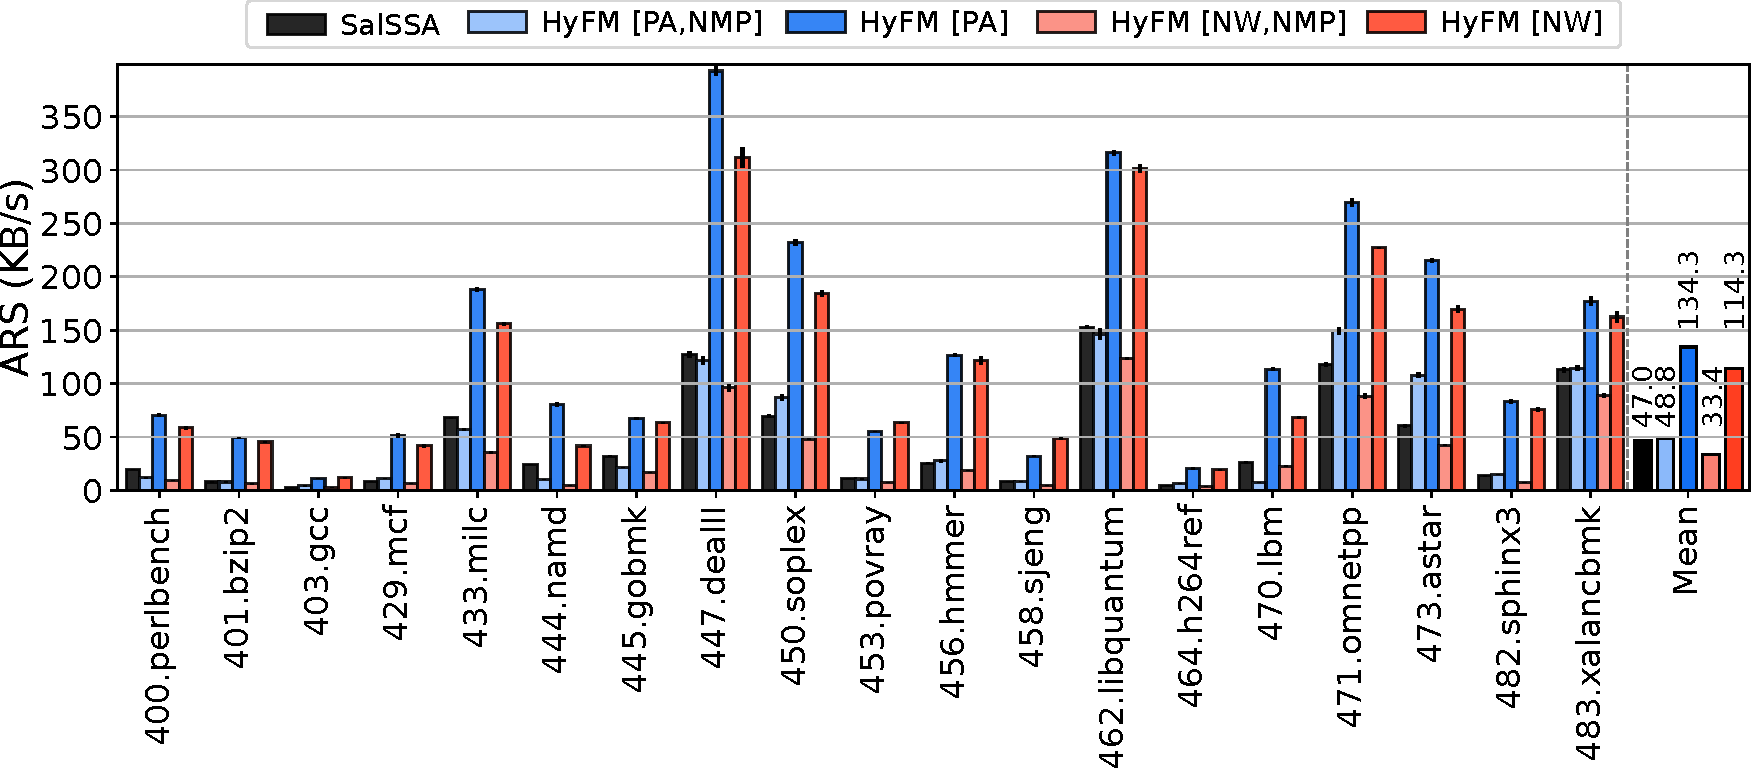
\includegraphics[width=\textwidth]{src/lctes21/figs/ars-spec06.pdf}
 \caption{SPEC CPU 2006.}
 \label{fig:ars-spec06}
 \end{subfigure}
 \\
 \begin{subfigure}{\textwidth}
 \center
   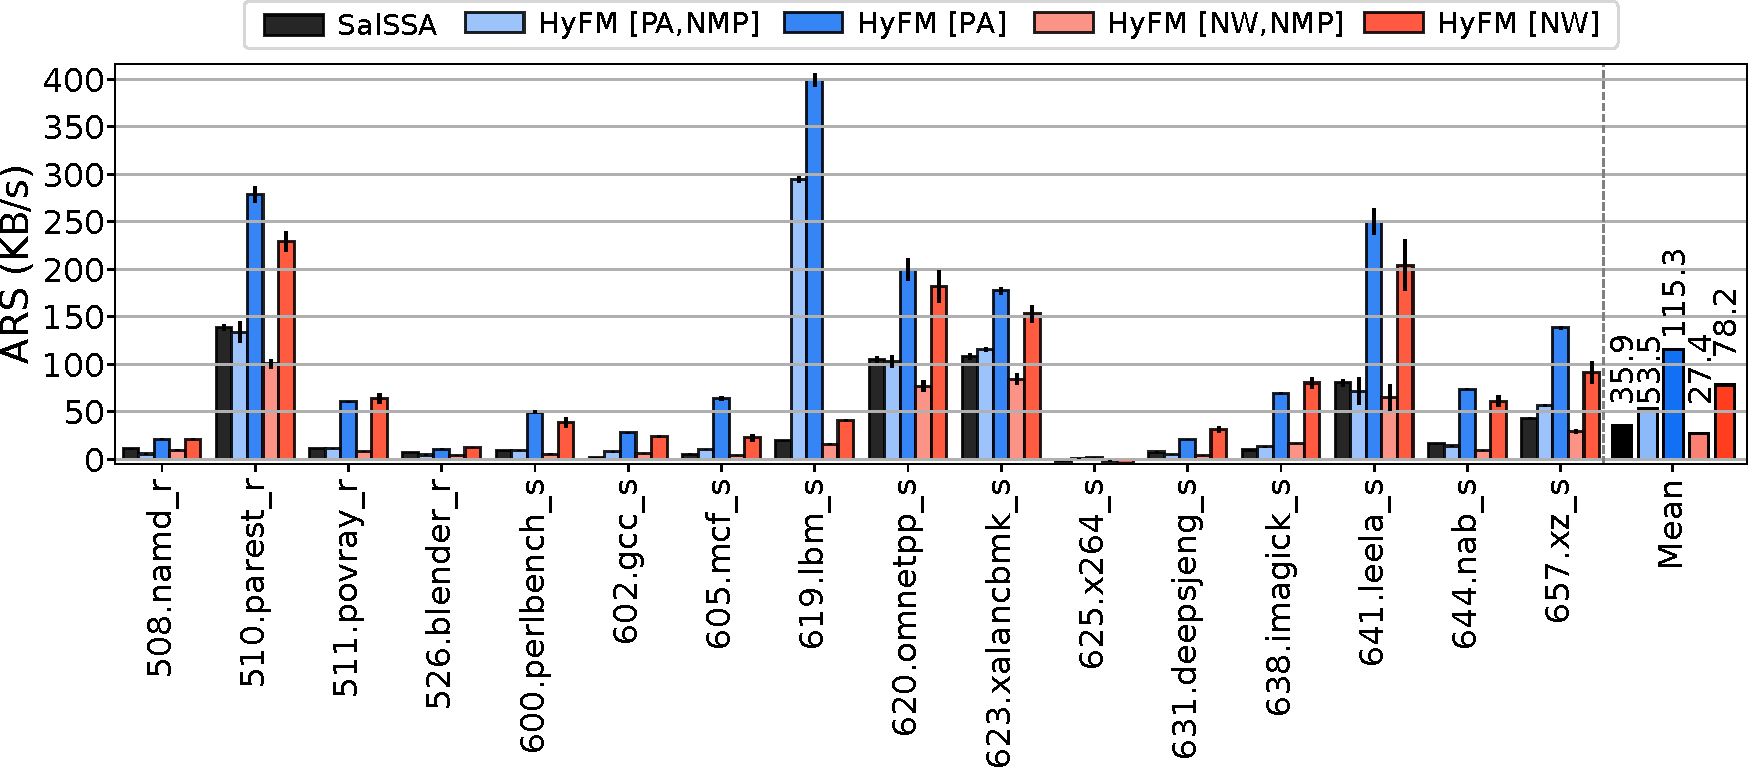
\includegraphics[width=\textwidth]{src/lctes21/figs/ars-spec17.pdf}
 \caption{SPEC CPU 2017.}
 \label{fig:ars-spec17}
 \end{subfigure}
 \caption{Average reduction speed on both SPEC 2006 and 2017.}
  \label{fig:ars-both}
 \end{figure}

%\begin{figure*}[h]
%  \centering
%  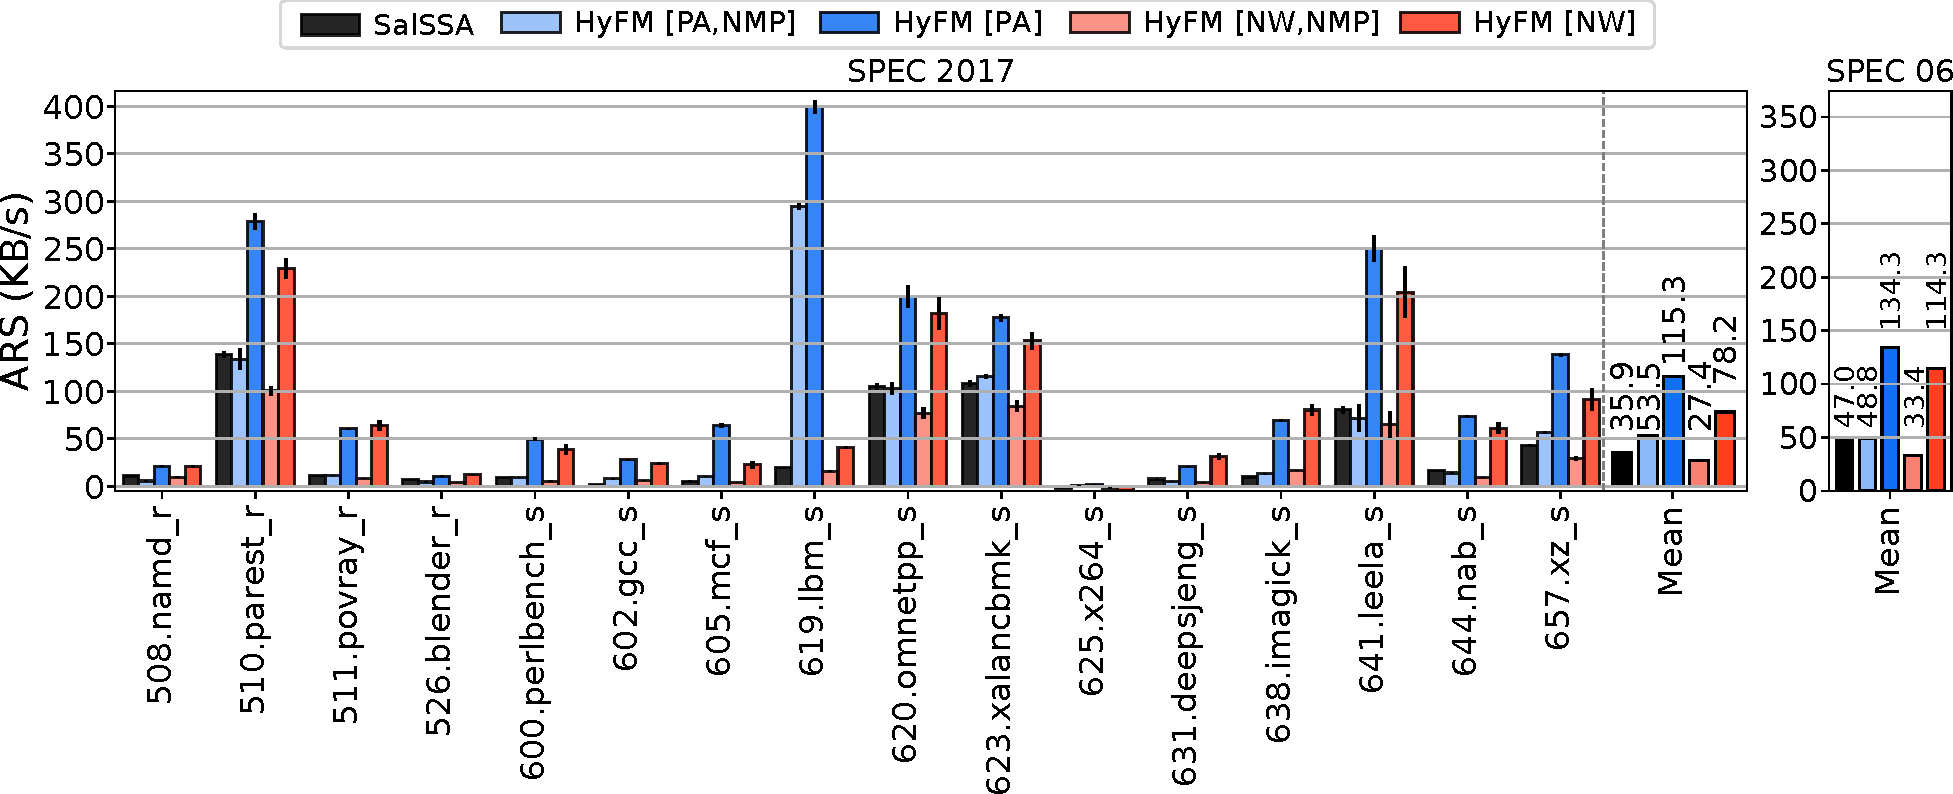
\includegraphics[width=0.95\linewidth]{src/lctes21/figs/ars-spec17-06.pdf}
%  \caption{Average reduction speed on both SPEC 2006 and 2017.}
%  \label{fig:ars-both}
%\end{figure*}

\subsection{Memory Usage} \label{sec:eval:memory}

 \begin{figure}[h]
   \centering
 \begin{subfigure}{\textwidth}
 \center
   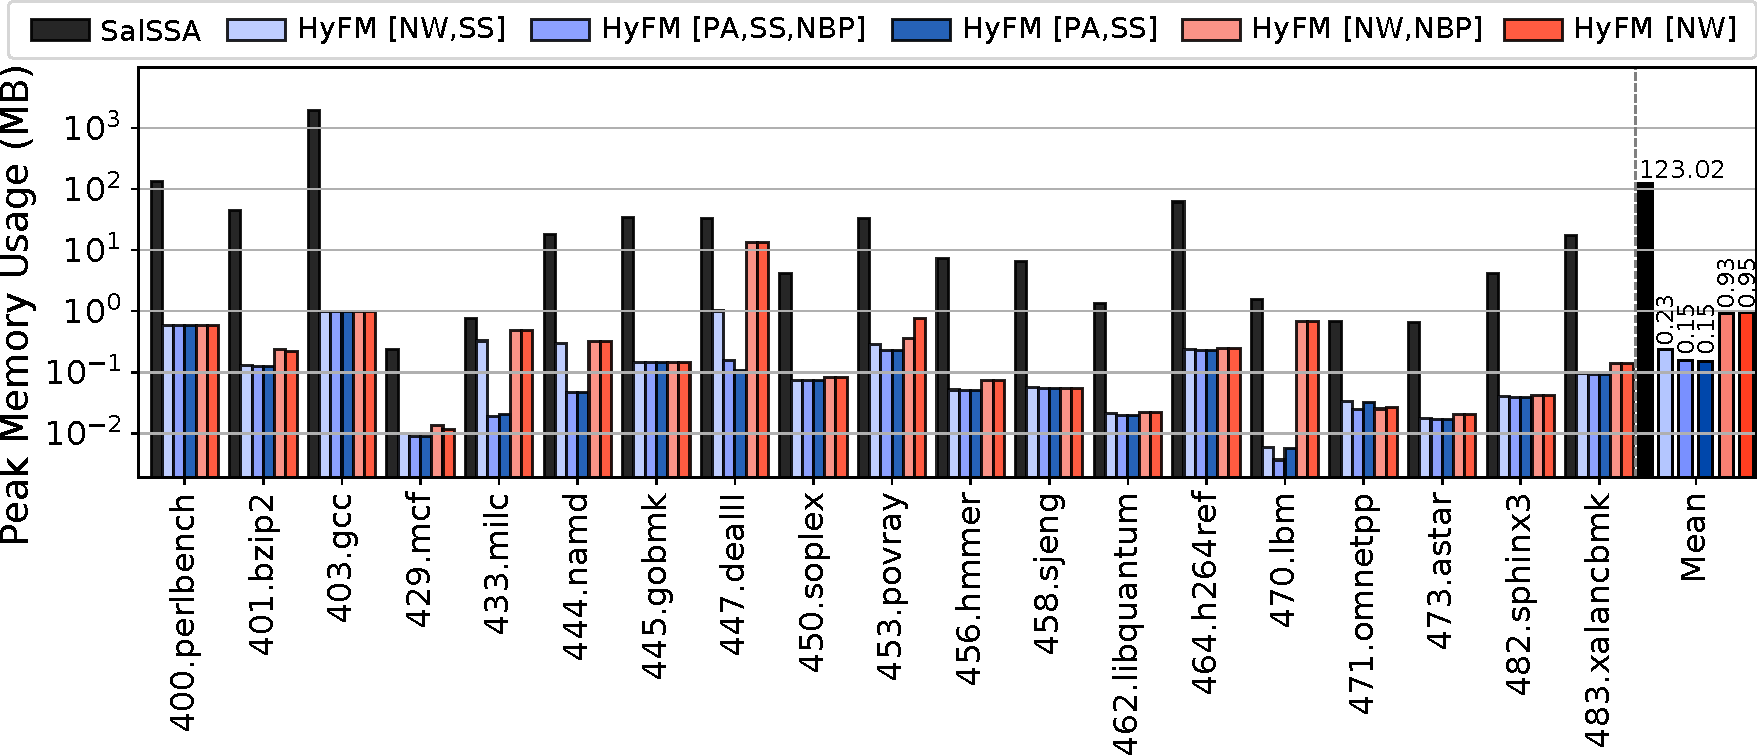
\includegraphics[width=\textwidth]{src/lctes21/figs/memory-spec06.pdf}
 \caption{SPEC CPU 2006.}
 \label{fig:memory-spec06}
 \end{subfigure}
 \\
 \begin{subfigure}{\textwidth}
 \center
   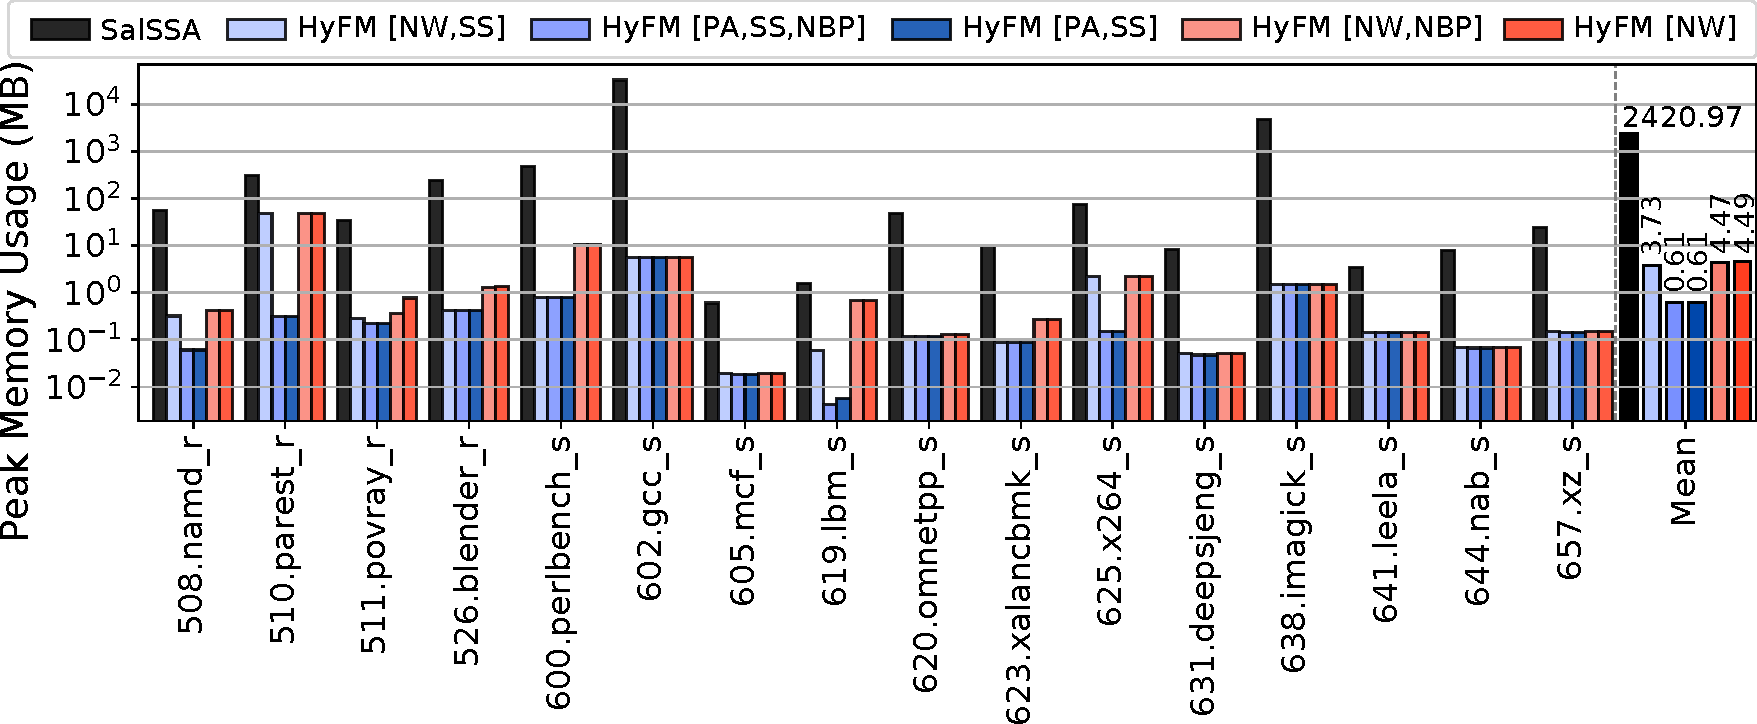
\includegraphics[width=\textwidth]{src/lctes21/figs/memory-spec17.pdf}
 \caption{SPEC CPU 2017.}
 \label{fig:memory-spec17}
 \end{subfigure}
 \caption{Peak memory usage of {\SOAName} and {\ProjName} variants for SPEC 2006 and 2017 in log scale. {\SOAName} has a peak memory usage several orders of magnitude hundreds higher than all other approaches. The pairwise alignment variants of {\ProjName} need on average only a seventh of the memory needed by the {\NW} variants.}
  \label{fig:memory-both}
 \end{figure}

%\begin{figure}[h]
%  \centering
%  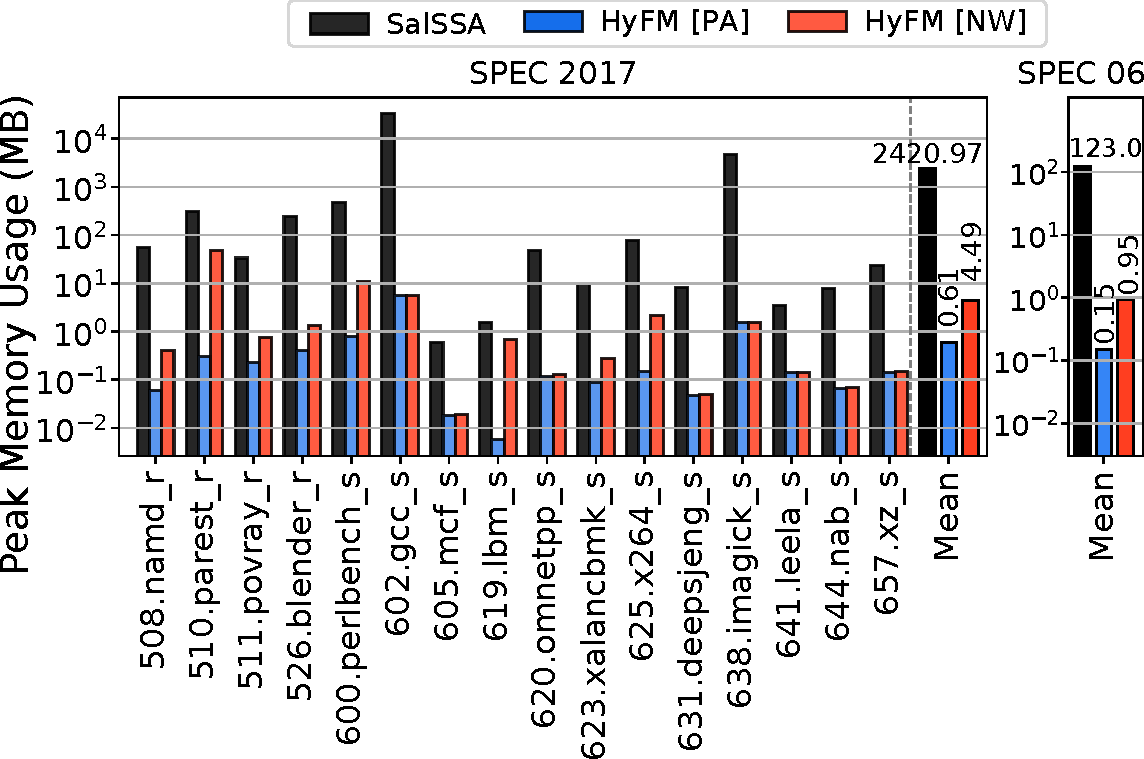
\includegraphics[width=\linewidth]{src/lctes21/figs/memory-spec17-06-tiny.pdf}
%  \caption{Peak memory usage of {\SOAName} and {\ProjName} variants for SPEC 2006 and 2017 in log scale. {\SOAName} has a peak memory usage several orders of magnitude hundreds higher than all other approaches. The pairwise alignment variants of {\ProjName} need on average only a seventh of the memory needed by the {\NW} variants.}
%  \label{fig:memory-both}
%\end{figure}

Another important aspect of function merging is peak memory usage. This is especially critical for an optimization designed for LTO.
Compilation in full LTO mode is already memory hungry. Just keeping the whole program in memory can be a significant problem for large programs~\cite{johnson17}. Maintaining additional information for every function and basic block could easily tip the compiler over the edge.

Figure~\ref{fig:memory-both} shows the peak memory usage (in log scale) needed for the alignment stage alone.
For {\SOAName}, this represents simply the execution of the {\NW} algorithm.
For {\ProjName}, the alignment stage represents both aligning each pair of basic blocks as well as the pairing these basic blocks.
Our results show that {[PA]} is over three orders of magnitude better than {\SOAName}, while {[NW]} is more than two orders of magnitude better.
In other words, while {\SOAName} requires on average 2.4~GB of memory, {[PA]} uses only around 610~KB and {[NW]} uses 5.6~MB.

The peak memory usage is especially noticeable on \texttt{gcc}, when merging its two largest functions, containing 90093 and 76265 instructions.
Since {\SOAName} applies its quadratic sequence alignment algorithm on the linearized sequences of the whole input functions, it uses over 32~GB of memory when merging these two functions.
Meanwhile, {[NW]} requires only around 5.6~MB for merging the same pair of input functions, even though it employs the same sequence alignment algorithm. This is because its peak memory usage is a quadratic function of the largest pair of \emph{blocks} instead of the largest pair of \emph{functions}.
Although very large, these two functions are composed of several thousands of very small basic blocks, so the memory overhead of {\NW} is limited.
Most of the memory consumed by {[NW]} in this case is actually needed for storing the basic block fingerprints.
This aspect becomes evident when we compare the peak memory usage of {[NW]} with that of the {[PA]} for \texttt{gcc}. They have similarly low memory requirements, even though only one of them uses a quadratic alignment algorithm.

In other cases, where basic blocks are longer, pairwise alignment leads to a significantly lower peak memory usage compared to {\NW}. For \texttt{parest}, for example, pairwise alignment reduces memory usage from \fixme{40}~MB to \fixme{200}~KB. Overall, {[PA]} needs around $6\times$ less memory. For smaller programs, {[NW]} might be a viable option but for larger ones being able to reduce memory usage to a minimum might be more important.

% \subsection{Summary}
% Overall, our novel function merging technique has surpassed the state-of-the-art in terms of compilation time, memory usage, as well as code size reduction.
% However, different variants of the proposed technique are better suited for different goals.
% If the code size is the utmost concern, {\ProjName}~[NW] is the winning strategy, but if we are looking for the most balanced trade-off between compilation-time overheads and code-size reduction, {\ProjName}~[PA] has shown better results.

\section{Conclusion}

% We have presented HyFM, a novel technique for compiler-based function merging. HyFM is designed to improve the scalability of the state-of-the-art function merging technique by reducing the compilation time and memory usage. HyFM provides a set of profitability analysis to enable function merging to be performed at the basic block level to reduce the compilation and memory overhead. It also allows the compiler to bail out early from unprofitable merging attempts to save compilation time

We have presented \ProjName, a novel technique for compiler-based function merging. By operating on individual pairs of basic blocks, it eliminates most of the time and space overheads of SalSSA. Through its multi-tier profitability analysis, it allows the compiler to bail out early from unprofitable merging attempts saving additional compilation time.

We evaluate \ProjName by applying it to SPEC CPU2006 and 2017 benchmark suites.
%Experimental results show that  \ProjName achieves comparable and often better results in code size reduction than the state-of-the-art. However, \ProjName achieves this while running over 4$\times$ faster and using orders of magnitude less memory. We further demonstrate how different variants of \ProjName can be developed, giving users the flexibility to control the trade-off between compilation overhead and code size reduction. 
Overall, \ProjName has surpassed SalSSA in terms of compilation time, memory usage, as well as code size reduction.
However, different variants of the proposed technique are better suited for different goals.
If the code size is the utmost concern, {\ProjName}~[NW] is the winning strategy, but if we are looking for the most balanced trade-off between compilation-time overheads and code-size reduction, {\ProjName}~[PA] has shown better results.

% Future work for improving function merging could focus on an even finer grain tier to the profitability analysis that works on individual pairs of aligned instructions. Another aspect that could be improved is the strategy for pairing functions, the most expensive part of function merging for some benchmarks.

